\documentclass[11pt,a4paper]{article}
\usepackage{fontspec}


\usepackage[margin=2.2cm]{geometry}
\usepackage{graphicx,booktabs,longtable,amsmath,amssymb,array,float,caption,xcolor}
\usepackage[hidelinks]{hyperref}
\renewcommand{\figurename}{Slika}
\renewcommand{\tablename}{Tabela}
\renewcommand{\contentsname}{Kazalo}
\renewcommand{\refname}{Viri}
\renewcommand{\abstractname}{Povzetek}
\definecolor{capc}{HTML}{4A2A6B}\captionsetup{font={small,color=capc},labelfont=bf,margin=1.2cm,justification=raggedright,singlelinecheck=true}
\setlength{\parskip}{0.4em}
\setlength{\parindent}{0pt}

\title{Odkrivanje potencialnih napak v preliminarnih\\rezultatih referendumov po voliščih\\z modelom štirih sočasnih referendumov}
\author{Tim Kmecl, dipl. inž. rač. in mat.}
\date{14.~oktober 2026}

\begin{document}
\maketitle

\begin{abstract}
\setlength{\parindent}{0pt}\setlength{\parskip}{0.5em}
\noindent Analiziral sem preliminarne (trenutne) rezultate štirih sočasnih referendumov (parlamentarna preiskava, RTV, sociala, tujci) na 3190 voliščih. Za vsak referendum delež glasov ZA na volišču napovem iz rezultatov ostalih treh referendumov na istem volišču. Ker gre za iste volivce, je napoved zelo natančna (bolj, kot to dopušča binomski šum med neodvisnimi vzorci), zato izstopajo tudi razmeroma majhna odstopanja. Med 12\,760 kombinacijami volišče\,$\times$\,referendum jih je 53 (na 50 voliščih) izstopajočih ($|z|>5$, po Gaussu pričakovano $<0{,}01$). Okoli polovica jih kaže vzorec, ki bi ga pričakovali pri zamenjavi rubrik ZA in PROTI: objavljeni rezultat je zrcalna vrednost napovedi, $100-\hat p$, do natančnosti binomskega šuma. 

\textbf{Najpomembnejša ugotovitev je, da se outlierji zgoščajo prav na zrcalni vrednosti napovedi, ki je za vsako volišče drugačna: tudi če bi outlierje pripisali resničnim lokalnim posebnostim volišč ali porazdelitvi z debelejšimi repi od predpostavljene, bi to pojasnilo njihovo število, težko pa zgoščevanje na območju, ki pripada zamenjavam.} Mešani model za vse outlierje (izbrane samo po $|z|>5$) oceni okoli 22 domnevnih zamenjav (95-\% IZ 15--30) in je s hipotezo ``samo resnične lokalne posebnosti, brez napak'' slabo skladen ($p<10^{-10}$); v isto smer kažejo test gladkosti brez modela ozadja in ničelni model z enako porazdelitvijo velikosti volišč. Nazoren primer: pri sedmih od osmih domnevnih zamenjav, kjer so v isti stavbi še druga volišča, ta glasujejo povsem v skladu z napovedjo ($|z|<2$), zgolj lokalna posebnost pa bi se verjetno pokazala tudi pri njih. Podoben primer je znan iz Danske, kjer so leta 2014 s primerjavo sočasnega referenduma in volitev po voliščih odkrili volišče z zamenjanima ZA in PROTI, kar je volilni organ potrdil.

Domnevne zamenjave so pogostejše na večjih voliščih (okoli 9 na milijon glasov), geografskega vzorca ni opaziti. Tudi če bi šlo za dejanske napake, na izid nobenega referenduma ne bi vplivale; največji relativni učinek bi bil pri RTV, kjer bi popravek označenih volišč povečal prednost PROTI s 546 na okoli 1400 glasov. Smer odstopanj vseh outlierjev (32 od 53 v škodo zmagovalca, pričakovano 27 brez zamenjav in 35--36 s samimi zamenjavami) je s tem skladna, a sama nima moči za ločevanje hipotez.

\textbf{Rezultati utemeljujejo sum, da gre pri približno 22 od 53 outlierjev za zamenjavo števil ZA in PROTI pri vpisu ali prepisu, vendar napak zgolj s statistično analizo ne moremo dokončno potrditi}. Da bi hipotezo z veliko zanesljivostjo potrdili ali ovrgli, zadošča že pregled zapisnikov in glasovnic na treh označenih voliščih z najmočnejšim signalom. Podatki ne kažejo znakov sistematičnega prirejanja.
\end{abstract}

\clearpage
\tableofcontents
\newpage

%=====================================================
\section{Podatki in izhodišče}

Podatki so rezultati po voliščih za štiri referendume, ki so potekali hkrati. Preneseni so bili v obliki Excel s spletne strani Državne volilne komisije (DVK) 13.\,10.\,2026 ob 19:30 (oznaka osvežitve podatkov v datotekah: 12.\,10.\,2026 ob 18:00). Analiza opisuje stanje podatkov ob prenosu; DVK je lahko katero od navedenih volišč medtem že popravila, zato se trenutno objavljeni rezultati lahko razlikujejo od tukaj analiziranih. Nacionalni deleži ZA v podatkih:

\begin{center}
\begin{tabular}{lrrr}
\toprule
Referendum & ZA \% & razlika (glasovi) & zmagovalec \\
\midrule
Parlamentarna preiskava & 48,74 & 23\,147 & PROTI \\
RTV & 49,97 & 546 & PROTI \\
Sociala & 60,54 & 194\,705 & ZA \\
Tujci & 55,30 & 97\,776 & ZA \\
\bottomrule
\end{tabular}
\end{center}

Gre za \textbf{preliminarne (trenutne) rezultate} in ne uradne rezultate: glasovi po pošti iz tujine so povsod 0, na nekaterih voliščih še niso bile preštete vse glasovnice. V analizo so vključena volišča z vsaj 10 veljavnimi glasovi pri vseh štirih referendumih (3190 volišč, vključno s predčasnim glasovanjem).

Povod za analizo je bila objava na družbenem omrežju, ki je opozorila na volišča z veliko razliko med rezultatoma preiskave in RTV ter namignila na nepravilnosti. Takšna primerjava dveh referendumov ne upošteva velikosti volišč, regionalnih razlik in tega, kateri od obeh rezultatov je napačen. Model štirih referendumov rešuje vse tri težave.

\subsection{Podobni primeri in metode}

Zamisel, da rezultate na volišču preverimo z rezultati drugih glasovanj na istem volišču, ni nova. Wand in sod.~\cite{wand2001} so po voliščih primerjali glasove za kandidata Buchanana na predsedniških volitvah v ZDA leta 2000 z glasovi za druge tekme na isti glasovnici in pokazali, da je nenavadno visok delež v okrožju Palm Beach posledica zmedne oblike glasovnice, ne pa dejanske podpore volivcev. Robustne regresijske metode za odkrivanje izstopajočih števil glasov po voliščih sta razvila Mebane in Sekhon~\cite{mebane2004}. Najbližji precedens tej analizi je primer z Danske: na dan evropskih volitev 2014 je potekal tudi referendum o Enotnem patentnem sodišču, in aktivisti organizacije Open Knowledge Denmark so po voliščih primerjali glasove ZA na referendumu z glasovi za stranke, ki so zagovarjale PROTI. Eno volišče (okoli 800 glasov) je izrazito izstopalo; volilni uradnik je še isti dan potrdil, da sta bila ZA in PROTI zaradi človeške napake zamenjana~\cite{okfn2014}. Tudi v sistemih z razvitimi kontrolami se napake pri vnosu pojavljajo: revizija novozelandskih volitev leta 2023 je odkrila napake, pri katerih so bili glasovi vpisani napačnim kandidatom ali strankam ali pa sta bila zamenjana rezultata predčasnega glasovanja in volilnega dne, na okoli 0,3--0,7~\% volišč~\cite{oagnz2024}. Ahlbäck in Jablonski~\cite{ahlback2025} sta na volitvah v Malaviju 2019 pokazala, da je bila večina popravkov v zapisnikih volišč posledica človeških napak in ne prevar, in da njihovo število naraste z zahtevnostjo štetja, kar je skladno z večjo pogostostjo domnevnih zamenjav na večjih voliščih v tej analizi (razdelek~\ref{sec:velikost}).


\subsection{Izrazi in kratice}
\label{sec:izrazi}

\textbf{Opomba o izrazih.} Analiza je statistična in temelji le na objavljenih številih. Kjer v besedilu zaradi jedrnatosti piše ``napaka'', ``zamenjava'' ali ``zamenjava ZA$\leftrightarrow$PROTI'', je vedno mišljena \emph{domnevna} napaka oziroma \emph{sum na} zamenjavo: volišče, katerega objavljeni rezultat se statistično ujema z vzorcem zamenjave. Poročilo ne trdi, da je na kateremkoli volišču napaka dejansko nastala; to je mogoče ugotoviti le s pregledom zapisnikov ali iz uradnih rezultatov.


\begin{itemize}\setlength{\itemsep}{0pt}
\item \emph{Celica}: kombinacija volišče $\times$ referendum (3190 volišč $\times$ 4 referendumi $=$ 12\,760 celic).
\item \emph{Outlier} (izstopajoča celica): celica, katere objavljeni rezultat od napovedi odstopa za več kot 5 standardnih odklonov ($|z|>5$).
\item \emph{logit}: preslikava deleža $p\in(0,1)$ na realno os, $\operatorname{logit}p=\ln\frac{p}{1-p}$; pogosto se uporablja pri regresiji deležev, ker napovedani delež vedno ostane med 0 in 1.
\item $z$: standardizirano odstopanje objavljenega deleža od napovedi (enačba~\ref{eq:z}); $z^{\text{zam}}$: enako, a za delež po zamenjavi ZA$\leftrightarrow$PROTI.
\item \emph{Razmik}: oddaljenost napovedi od 50~\% v enotah šuma, $(1-2\hat p)/\text{šum}$; zamenjava je zaznavna le pri dovolj velikem razmiku.
\item $\lambda$: položaj objavljenega rezultata med napovedjo ($\lambda=0$) in njeno zrcalno vrednostjo ($\lambda=1$), enačba~\ref{eq:lambda}.
\item $\pi$: delež zamenjav med outlierji v mešanem modelu (razdelek~\ref{sec:lambda}); $\pi=0$ pomeni, da zamenjav ni.
\item \emph{FE} (fiksni učinki): dodatni člen v modelu za vsak volilni okraj, ki zajame povprečni odklon okraja.
\item \emph{MAD} (mediana absolutnih odklonov): robustna mera razpršenosti, na katero posamezni outlierji ne vplivajo.
\item $R^2$: delež razlik med volišči, ki ga pojasni napoved; \emph{RMSE}: koren povprečnega kvadrata odstopanja napovedi (tipična velikost odstopanja).
\item \emph{IZ}: interval zaupanja; \emph{o.\,t.}: odstotne točke; $\sigma$: standardni odklon.
\item \emph{Mann-Whitney} (MW) in \emph{Kolmogorov-Smirnov} (KS): testa, ali dve skupini izhajata iz iste porazdelitve; $\chi^2$: hi-kvadrat test; $p$: verjetnost, da bi bil rezultat vsaj tako izrazit, če velja ničelna hipoteza.
\end{itemize}

%=====================================================
\section{Model}

\subsection{Zakaj štirje referendumi}

Na istem volišču glasujejo isti volivci o štirih vprašanjih. Deleži ZA so med volišči močno povezani: uteženi korelacijski koeficienti so 0,95--0,98, in tudi znotraj istega volilnega okraja (po odštetju povprečja okraja) ostanejo 0,93--0,96 (sliki~\ref{fig:korm} in~\ref{fig:korh}). Volišče je torej samo sebi najboljša referenca: rezultat enega referenduma lahko napovemo iz ostalih treh veliko natančneje kot iz povprečja okraja.

Ključna lastnost: splošni lokalni premik (``bolj levo'' ali ``bolj desno'' volišče) se pokaže pri vseh štirih referendumih hkrati in se v napovedi izniči. Napaka v zapisniku ali pri vnosu pa prizadene en sam referendum.

\begin{figure}[p]
\centering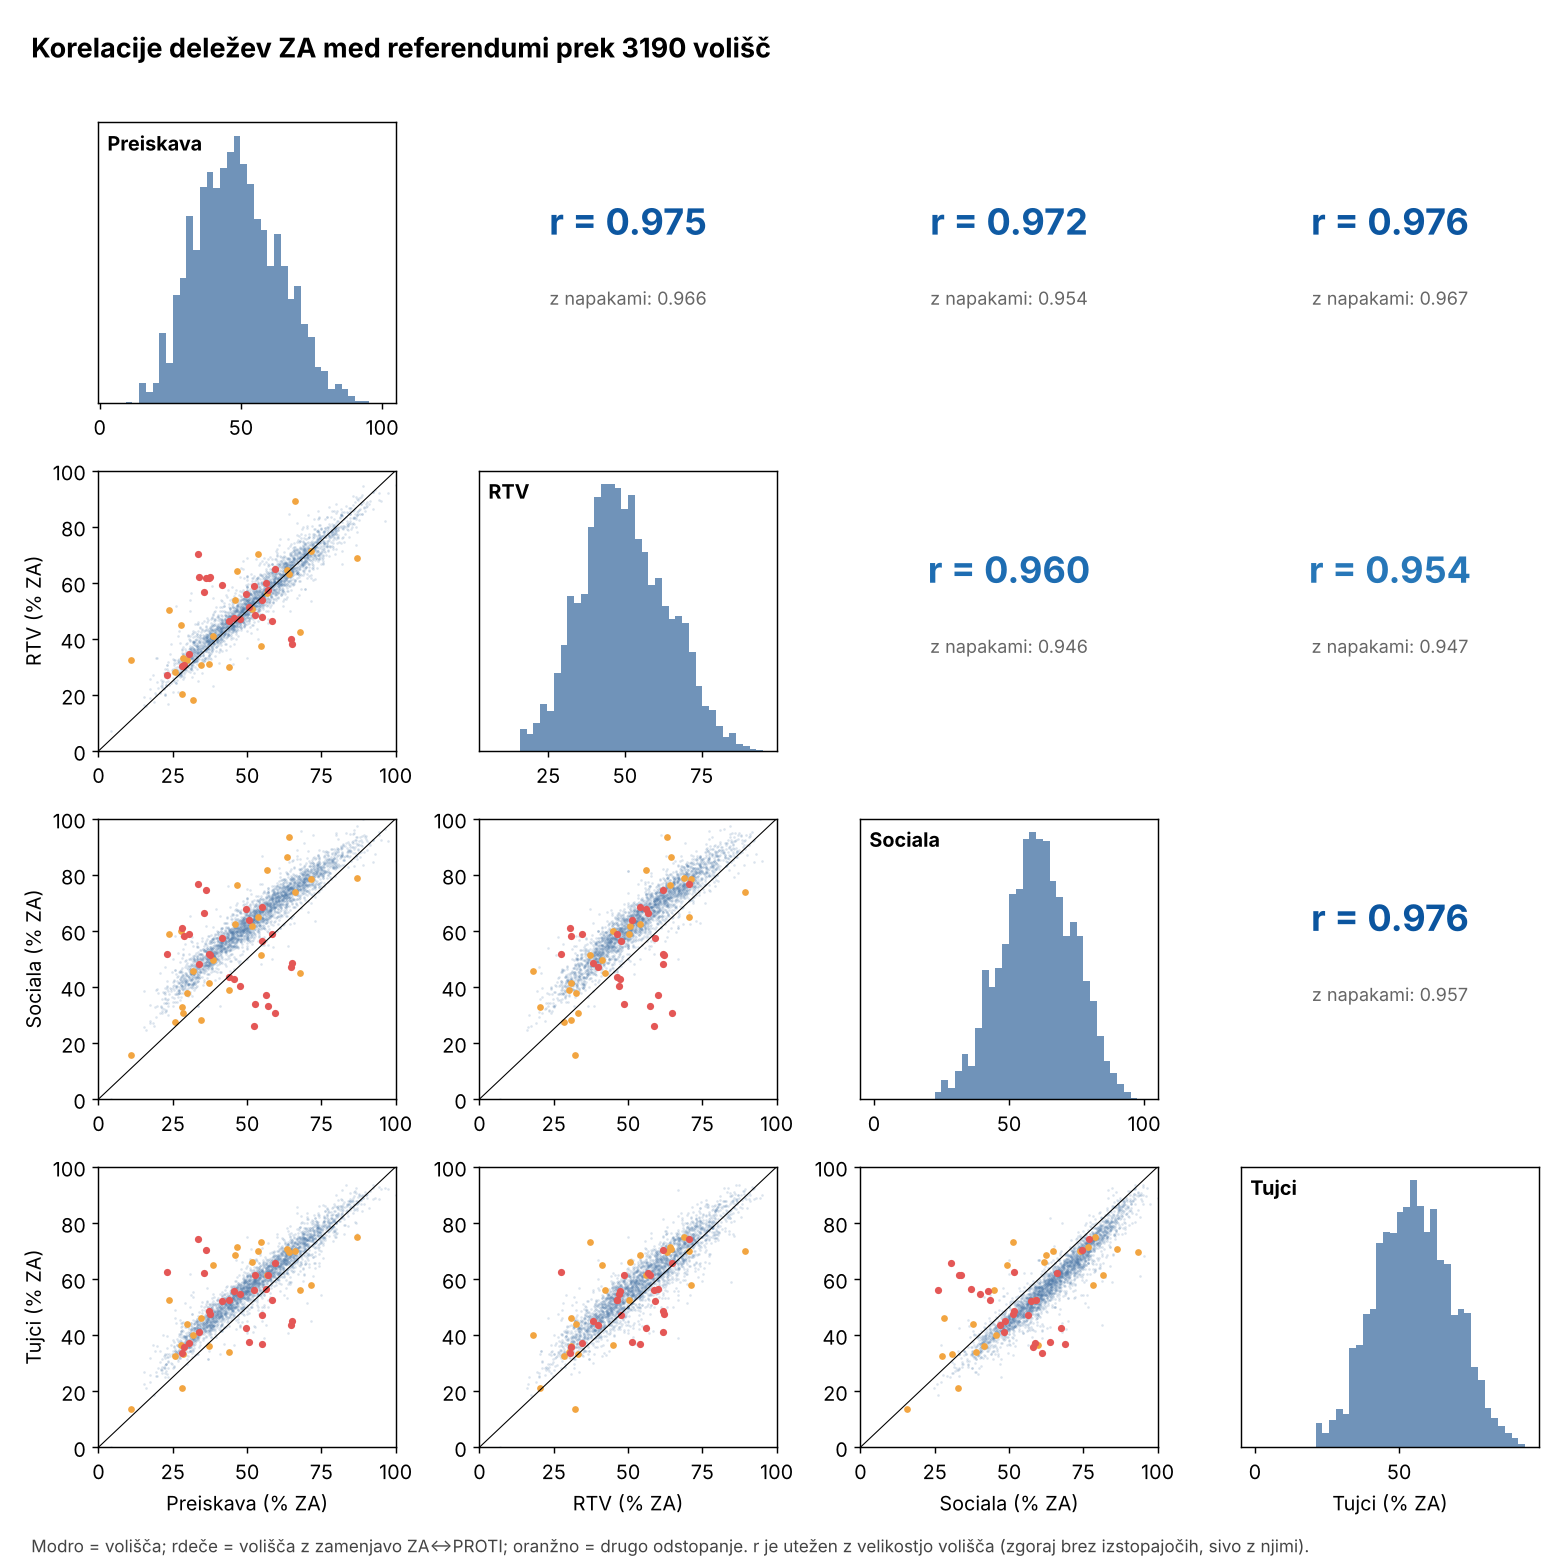
\includegraphics[width=0.6\textwidth]{6_korelacije_matrika.png}
\caption{Deleži ZA med pari referendumov; vsaka točka je volišče (3190 volišč). Diagonala: oba deleža enaka. Na diagonali so histogrami deležev ZA posameznega referenduma, nad njo uteženi korelacijski koeficienti $r$ (velika številka brez izstopajočih volišč, manjša z njimi). Modro: volišča; rdeče: volišča z domnevno zamenjavo ZA$\leftrightarrow$PROTI; oranžno: drugi outlierji. Volišča z zamenjavo izstopajo iz sicer zelo ozkega oblaka.}
\label{fig:korm}

\vspace{0.8em}
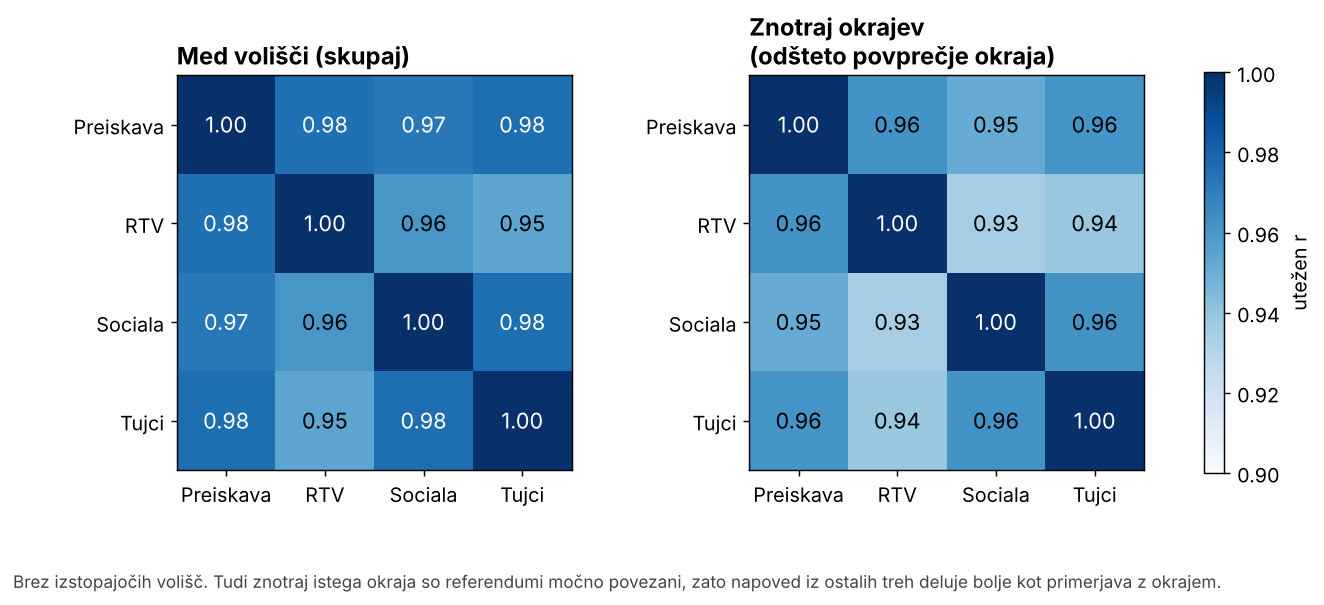
\includegraphics[width=0.72\textwidth]{7_korelacije_heatmap.png}
\caption{Uteženi korelacijski koeficienti deležev ZA med referendumi (utež: število glasov). Levo prek vseh volišč, desno znotraj okrajev, ko od deleža volišča odštejemo povprečje njegovega okraja. Izstopajoča volišča so izključena. Tudi znotraj okrajev so korelacije 0,93--0,96, zato ostali trije referendumi napovedo rezultat bolje kot povprečje okraja.}
\label{fig:korh}
\end{figure}

\subsection{Napoved}

Za vsak referendum $k$ in volišče $i$ ocenim regresijo v logitih:
\begin{equation}
\operatorname{logit}\hat p_{ik} = \beta_{0k} + \sum_{j\neq k}\beta_{jk}\,\operatorname{logit} p_{ij},
\label{eq:model}
\end{equation}
kjer je $p_{ij}$ objavljeni delež ZA na volišču $i$ pri referendumu $j$ in $\hat p_{ik}$ napoved za referendum $k$. Uteži so $w_{ik}=n_{ik}\,p_{ik}(1-p_{ik})$ (inverzna varianca deleža, $n_{ik}$ je število veljavnih glasov). Ocena je robustna (Huberjeva funkcija izgube, iterativno prevrednotenje uteži), da outlierji ne vplivajo na koeficiente. Model ocenim dvakrat: brez in s fiksnimi učinki okraja (FE); pri slednjem desni strani enačbe~\ref{eq:model} prištejem še člen $\gamma_{k,\text{okraj}(i)}$, ki je za vsak okraj drugačen.

\textbf{Dvostopenjsko čiščenje.} Napovedovalci so lahko tudi sami napačni (če je na volišču napaka pri preiskavi, pokvari napoved za ostale tri). Zato:
\begin{enumerate}
\item \emph{Robustna predhodna napoved}: za vsak $k$ ocenim tri modele z enim samim napovedovalcem in vzamem mediano njihovih napovedi. Ena napaka ne more premakniti mediane treh.
\item Na vsakem volišču, kjer kateri $|z|>5$, celico z največjim odstopanjem nadomestim s predhodno napovedjo, vendar \emph{samo v vlogi napovedovalca}.
\item \emph{Končna napoved}: polni model s tremi napovedovalci na očiščenih podatkih.
\end{enumerate}
Korak 2 služi izključno temu, da morebitna napaka v eni celici ne pokvari napovedi za ostale tri referendume na istem volišču. Nadomeščena vrednost se nikoli ne uporabi kot ciljna spremenljivka: odstopanje $z_{ik}$ vsake celice, tudi nadomeščene, je v končnem koraku vedno izračunano iz \emph{objavljenega} deleža $p_{ik}$ in napovedi iz ostalih treh referendumov. Razvrstitev med outlierje in zamenjave temelji samo na končnem koraku, predhodni $z$ iz koraka 1 se zanjo ne uporablja.

\textbf{Preverjanje krožnosti.} Predhodna napoved celice $(i,k)$ je mediana treh napovedi, med katerimi je tudi napoved iz referenduma $j$. Ko nadomeščeno vrednost uporabimo za napoved $j$, lahko ta posredno vsebuje informacijo o $j$ samem in napoved rahlo potegne k objavljeni vrednosti (to bi bilo konzervativno, saj bi zmanjšalo odstopanja). Zato sem postopek ponovil tako, da je pri napovedi referenduma $j$ nadomestna vrednost izračunana brez uporabe $j$ (povprečje napovedi iz preostalih dveh referendumov). Množica 53 outlierjev in 26 domnevnih zamenjav ostane popolnoma enaka; največja sprememba $z$ katerekoli celice je 1,6, pri le 13 od 12\,760 celic je večja od 0,5.

\subsection{Standardizirano odstopanje}

\begin{align}
z_{ik} &= \frac{p_{ik}-\hat p_{ik}}{c_k\sqrt{\hat p_{ik}(1-\hat p_{ik})/n_{ik}}}, \label{eq:z}\\
z^{\text{zam}}_{ik} &= \frac{(1-p_{ik})-\hat p_{ik}}{c_k\sqrt{\hat p_{ik}(1-\hat p_{ik})/n_{ik}}}. \label{eq:zzam}
\end{align}
Imenovalec je binomski šum, ki upošteva velikost volišča. Faktor $c_k$ je robustna ocena dejanske razpršenosti (MAD, normalizirana), ocenjena iz podatkov:

\begin{center}
\begin{tabular}{lcccc}
\toprule
 & Preiskava & RTV & Sociala & Tujci \\
\midrule
$c_k$ brez FE & 0,75 & 1,01 & 0,85 & 0,81 \\
$c_k$ s FE & 0,69 & 0,84 & 0,77 & 0,70 \\
\bottomrule
\end{tabular}
\end{center}

$c_k<1$ pomeni, da je napoved iz istih volivcev natančnejša od binomskega šuma med neodvisnimi vzorci. $z^{\text{zam}}$ je odstopanje, ki bi ga dobili, če bi na tej celici zamenjali ZA in PROTI.

Napoved pojasni 95--98~\% razlik med volišči (utežen $R^2$ 0,95--0,98 brez fiksnih učinkov, 0,97--0,98 z njimi), tipično odstopanje objavljenega deleža od napovedi pa je 2--3 odstotne točke (uteženi RMSE; mediana absolutnega odstopanja 1,5--2 o.\,t.). To je primerljivo z binomskim šumom zaradi končnega števila volivcev (okoli 2,8 o.\,t.), zato ni pričakovati, da bi bila napoved lahko bistveno natančnejša. Vrednosti so izračunane brez 53 outlierjev; z njimi je $R^2$ nižji za 0,01--0,03.

\subsection{Pravila za razvrščanje}
\begin{itemize}
\item \textbf{Outlier}: $|z|>5$ v obeh modelih (brez in s FE).
\item \textbf{Zamenjava ZA$\leftrightarrow$PROTI}: outlier, pri katerem je $|z^{\text{zam}}|<3$ v obeh modelih.
\item \textbf{Več referendumov}: na istem volišču izstopa več referendumov, zamenjava ne pomaga.
\item \textbf{Nepojasnjeno}: ostalo.
\end{itemize}

%=====================================================
\section{Rezultati}

\subsection{Porazdelitev odstopanj}

Jedro porazdelitve $z$ je pri vseh štirih referendumih normalno (kurtoza za $|z|<4$ med 0,2 in 0,5), napake pa tvorijo ločen rep (slika~\ref{fig:qq}, levo). Lijakasti prikaz (slika~\ref{fig:qq}, desno) pokaže, da outlierji niso posledica majhnih volišč: večinoma so na voliščih s 100--1000 glasovi, kjer je šum majhen.

\begin{center}
\begin{tabular}{lcccc}
\toprule
 & $|z|>3$ & $|z|>4$ & $|z|>5$ & \\
\midrule
Pričakovano (Gauss, na referendum) & 8,6 & 0,20 & 0,002 & \\
Preiskava (brez FE / s FE) & 44 / 43 & 24 / 22 & 15 / 18 & \\
RTV & 30 / 34 & 14 / 15 & 11 / 12 & \\
Sociala & 42 / 46 & 25 / 27 & 18 / 22 & \\
Tujci & 45 / 55 & 18 / 22 & 12 / 14 & \\
\bottomrule
\end{tabular}
\end{center}

Oba modela se skoraj popolnoma ujemata: 53 celic je izstopajočih v obeh, model s FE doda 13 mejnih, model brez FE 3. Fiksni učinek okraja skoraj nič ne spremeni, ker ostali trije referendumi že zajamejo lokalni profil volišča.

\begin{figure}[H]
\centering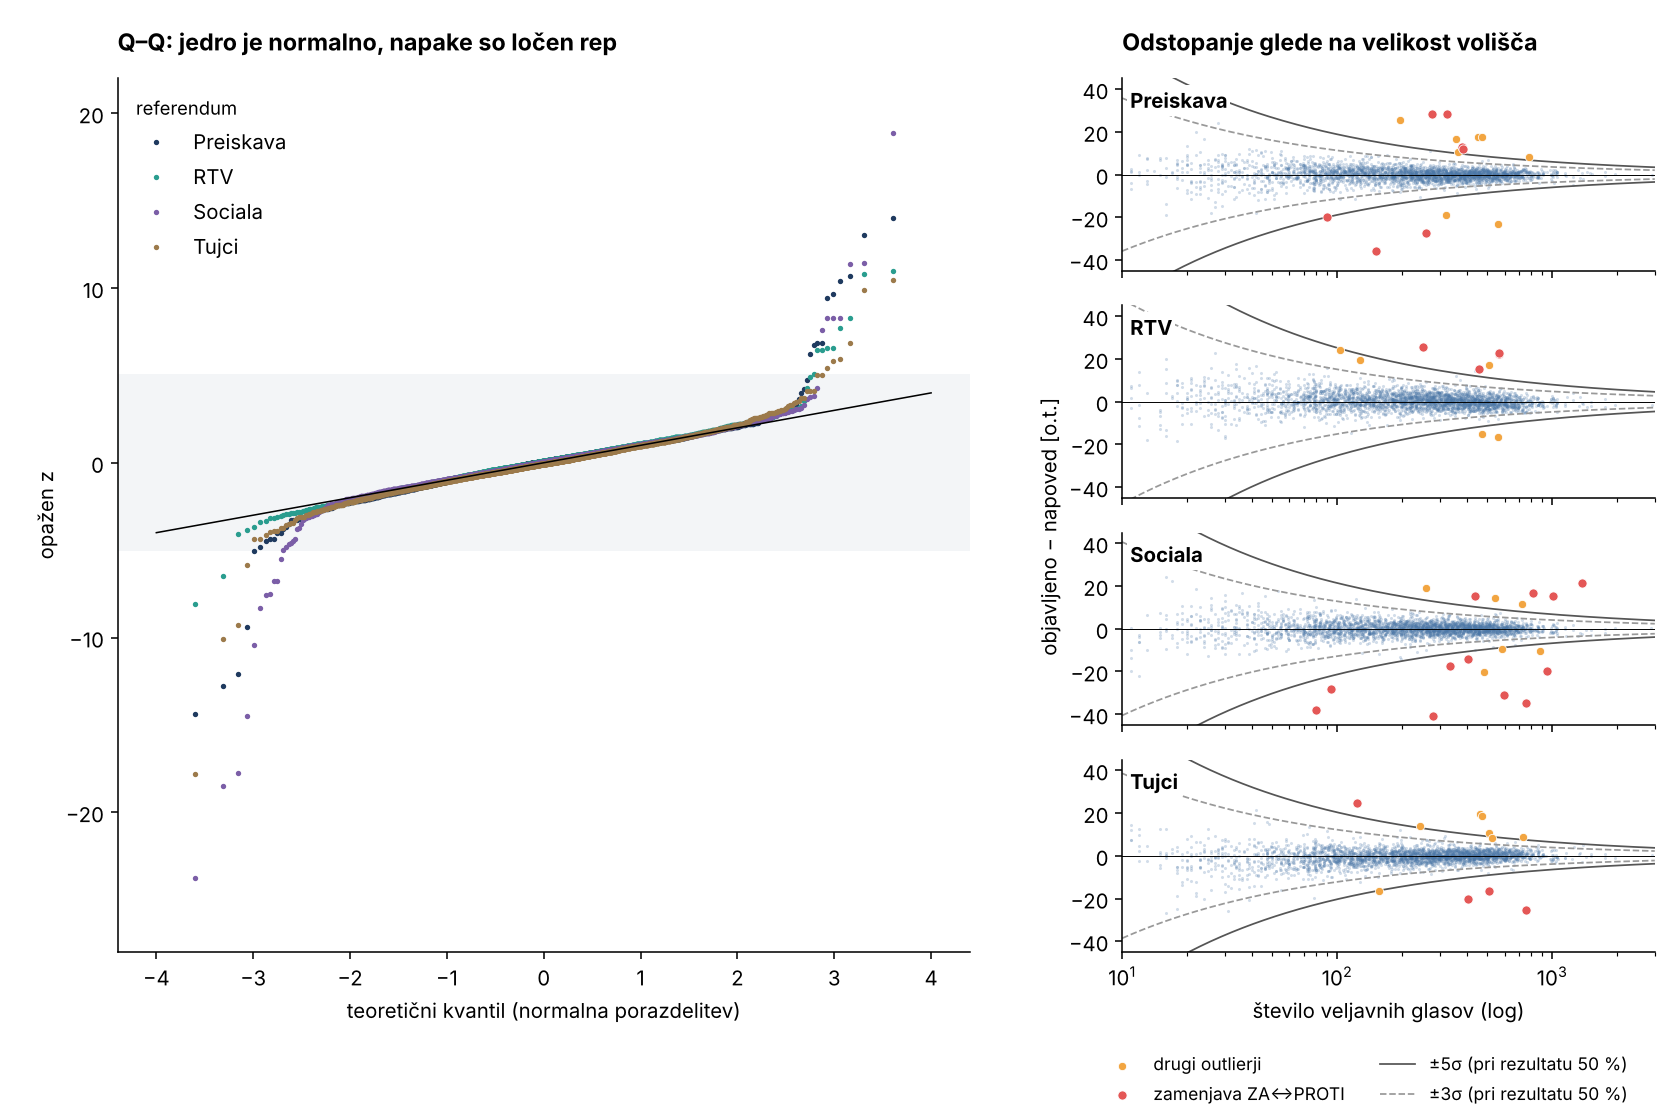
\includegraphics[width=\textwidth]{4_qq_lijak.png}
\caption{Levo: Q--Q diagram, urejena opažena odstopanja $z$ (navpično) proti kvantilom standardne normalne porazdelitve (vodoravno), za vsak referendum posebej. Če bi bila odstopanja normalna, bi točke ležale na črni premici. Jedro ($|z|\lesssim3$) leži na premici, outlierji pa tvorijo ločena repa, ki ju normalna porazdelitev ne predvideva; sivi pas označuje $|z|<5$. Desno: lijakasti prikaz, odstopanje objavljenega deleža od napovedi (v odstotnih točkah) glede na število veljavnih glasov na volišču. Pričakovani šum se z velikostjo volišča zmanjšuje, zato so meje $\pm3\sigma$ in $\pm5\sigma$ v obliki lijaka; večja odstopanja normalnih volišč so pri majhnih voliščih, outlierji pa ležijo zunaj lijaka. Meji sta narisani za rezultat 50~\%, kjer je šum največji; nekaj outlierjev z napovedjo daleč od 50~\% zato leži tik znotraj meje.}
\label{fig:qq}
\end{figure}

\begin{figure}[H]
\centering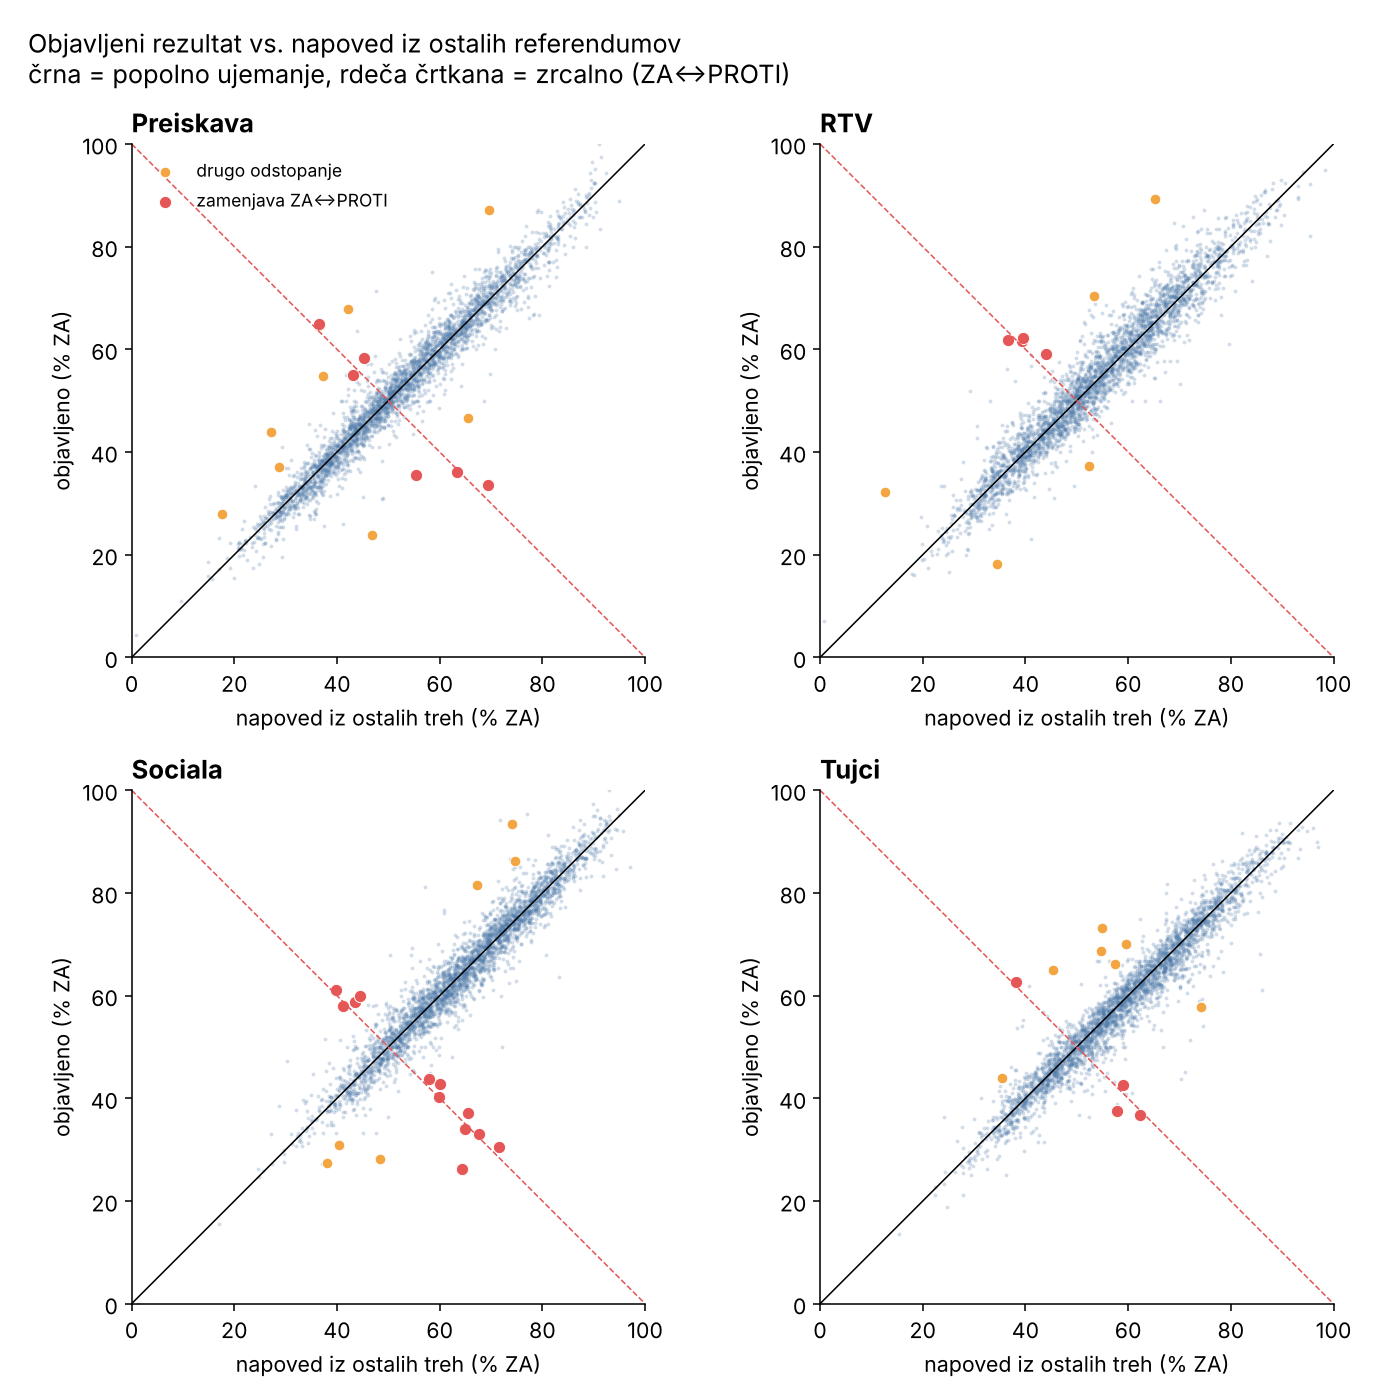
\includegraphics[width=0.85\textwidth]{1_napoved_vs_objavljeno.png}
\caption{Objavljeni delež ZA (navpično) proti napovedi iz ostalih treh referendumov (vodoravno), za vsak referendum posebej; vsaka točka je volišče. Črna diagonala: objavljeno $=$ napoved; rdeča črtkana: zrcalna črta, objavljeno $=100-$napoved (kjer bi ležala volišča z zamenjanima ZA in PROTI). Rdeče: domnevne zamenjave ZA$\leftrightarrow$PROTI; oranžno: drugi outlierji ($|z|>5$). Outlierji se zgoščajo ob zrcalni črti, kar je najbolje vidno pri sociali, kjer leži večina outlierjev prav na njej. Nekatere normalne (modre) točke so od diagonale bolj oddaljene kot najmanj oddaljeni outlierji; to so večinoma majhna volišča z večjim šumom (glej prejšnjo sliko).}
\label{fig:napoved}
\end{figure}

\subsection{Razvrstitev outlierjev}\label{sec:razvrstitev}

Od 53 izstopajočih celic na 50 voliščih:
\begin{itemize}
\item \textbf{26} čistih zamenjav ZA$\leftrightarrow$PROTI (preiskava 7, RTV 4, sociala 11, tujci 4);
\item \textbf{1} morda zamenjava;
\item \textbf{5} celic na dveh voliščih z odstopanjem pri več referendumih (OŠ Sostro, Moste-Polje~1/25: preiskava, RTV in tujci; Škofja Loka~1/6: RTV in tujci);
\item \textbf{21} nepojasnjenih.
\end{itemize}

Pri vseh izstopajočih voliščih je število oddanih glasovnic med štirimi referendumi skladno (razlika 0--1, največ 5). Napake so torej v razdelitvi glasov na ZA in PROTI, ne v številu glasovnic.

\begin{figure}[H]
\centering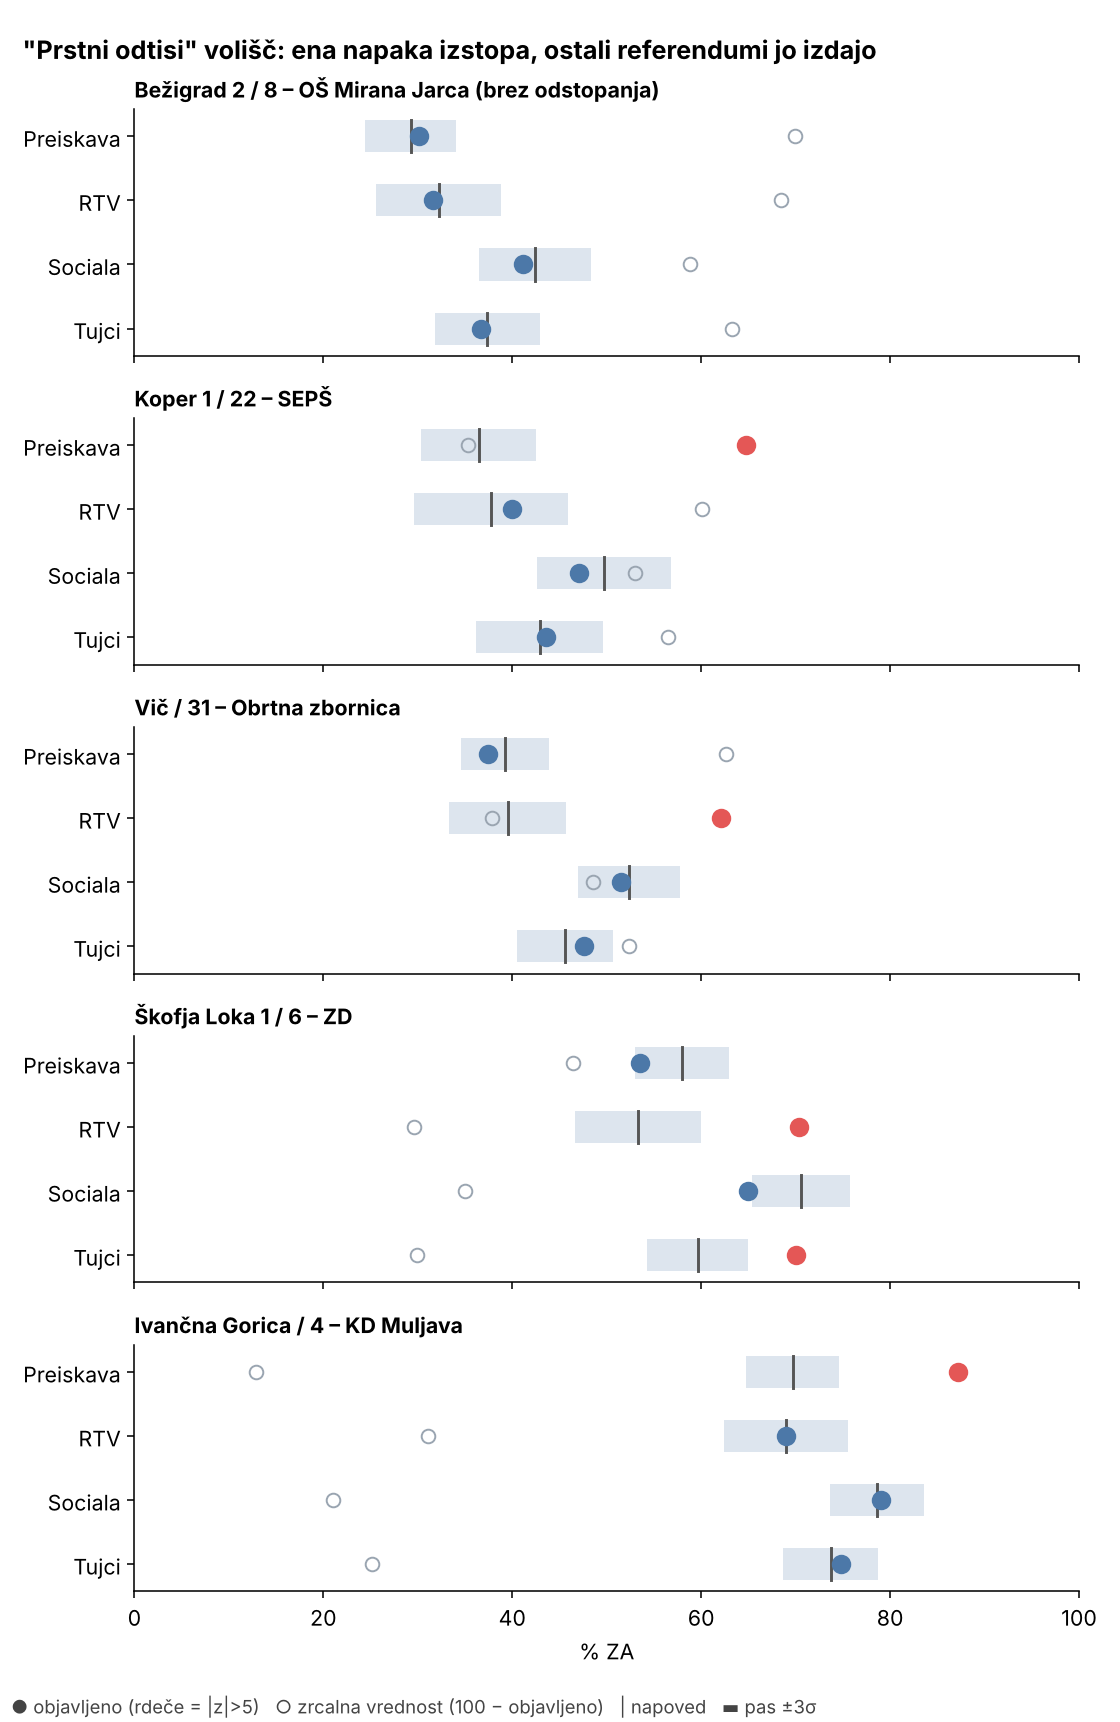
\includegraphics[width=0.75\textwidth]{3_prstni_odtisi.png}
\caption{``Prstni odtisi'' petih izbranih volišč. Za vsak referendum: objavljeni delež ZA (poln krog; rdeč, če je $|z|>5$), njegova zrcalna vrednost $100-p$ (prazen krog), napoved iz ostalih treh referendumov (navpična črta) in pas $\pm3$ standardnih odklonov okoli napovedi (siv pravokotnik). Bežigrad~2/8 (OŠ Mirana Jarca): tipično volišče brez odstopanja, vsi objavljeni rezultati so v pasu okoli napovedi, zrcalne vrednosti pa daleč od nje. Koper~1/22 in Vič/31: izstopa en referendum, njegova zrcalna vrednost pa pade na napoved (domnevna zamenjava ZA$\leftrightarrow$PROTI). Škofja Loka~1/6: izstopata dva referenduma, zamenjava odstopanja ne pojasni. Ivančna Gorica/4 (KD Muljava): izstopa en referendum, vendar odstopa stran od 50~\%, zato zamenjava ne pomaga (nepojasnjen outlier).}
\label{fig:prst}
\end{figure}

\subsection{Večkratne zamenjave na istem volišču}\label{sec:veckratne}

Za vsako volišče sem preizkusil vseh 16 kombinacij zamenjav (vsak referendum zamenjan ali ne) in izbral kombinacijo z najmanjšo vsoto $\sum_k z_k^2$. Najizrazitejši primer domnevne večkratne zamenjave je \textbf{Maribor~5/17, OŠ Draga Kobala}: objavljeni deleži ZA 68 / 42 / 45 / 56 \%; po zamenjavi pri preiskavi, sociali in tujcih 32 / 42 / 55 / 44 \%, kar se ujema z okrajem (41 / 44 / 56 / 50). Vsota $z^2$ pade s 157 na 13 (pri zamenjavi samo preiskave le na 67). Možen dvojni primer je Žalec~2/37 (sociala zelo verjetno, RTV pri 48 \% ni mogoče potrditi). Večkratne zamenjave je mogoče zaznati le, kadar so vsi prizadeti referendumi dovolj daleč od 50~\%.

\subsection{Velikost volišč in geografija}
\label{sec:velikost}

Zamenjave so na izrazito večjih voliščih (slika~\ref{fig:velikost}). Ker so na velikih voliščih zamenjave lažje zaznavne (manjši šum), primerjam le z ``zaznavnimi'' celicami, kjer bi zamenjava dala $|z|>5$ (razmik med normalo in zrcalno osjo $>5\sigma$; 24 od 26 zamenjav).

\begin{center}
\begin{tabular}{lrcc}
\toprule
 & celic & mediana glasov & kvartili \\
\midrule
zaznavne celice & 8\,610 & 258 & 131--431 \\
zamenjave & 26 & \textbf{394} & 264--590 \\
drugi outlierji & 27 & 471 & 338--550 \\
\bottomrule
\end{tabular}
\end{center}

Razlika med zamenjavami in zaznavnimi celicami je značilna (Mann-Whitney $p=0{,}004$, KS $p=0{,}014$). Po kvintilih velikosti je opaženih 2 / 2 / 4 / 6 / 10 zamenjav. Hipoteza ``enaka verjetnost napake na volišče'' (4,8 na kvintil) je zavrnjena ($\chi^2$, $p=0{,}05$), hipoteza ``verjetnost sorazmerna s številom glasov'' (1,1 / 2,4 / 4,0 / 6,1 / 10,3) pa se ujema skoraj popolno ($p=0{,}95$). Stopnja je okoli 9 domnevnih zamenjav na milijon glasov v zaznavnih celicah. Predčasna glasovanja so med zamenjavami nadpovprečno zastopana (11,5~\% proti 5,5~\%), kar je skladno s tem, da so to praviloma velika volišča.

Sorazmernost s številom glasov je skladna s človeško napako pri štetju in vpisu: na večjem volišču je glasovnic več, štetje traja dlje, volilni odbor rezultate praviloma sporoči pozneje in pogosto pozno zvečer, ko je utrujenost večja. Ta razlaga je verjetna, ni pa preverjena, ker podatki ne vsebujejo časa sporočanja rezultatov.

\textbf{Geografija} (ocena po imenih krajev). Po volilnih enotah so zamenjave razporejene enakomerno (Kranj 4, Postojna 3, Ljubljana Center 2, Ljubljana Bežigrad 4, Celje 4, Novo mesto 4, Maribor 0 + trojna zamenjava v Mariboru~5/17, Ptuj 5). Po tipu okolja je okoli 7 mestnih ali primestnih, 7 v manjših mestih ali predčasnih glasovanjih na upravnih enotah in 12 podeželskih. Podeželskih je nekaj manj od deleža podeželskih volišč, kar je skladno z učinkom velikosti. Edina zgostitev so trije primeri v okraju Murska Sobota~1, kar po naključju ni nenavadno ($p\approx0{,}31$). Velikost volišča (število veljavnih glasovnic) je edini dejavnik, ki statistično pojasni razporeditev domnevnih zamenjav.

\begin{figure}[H]
\centering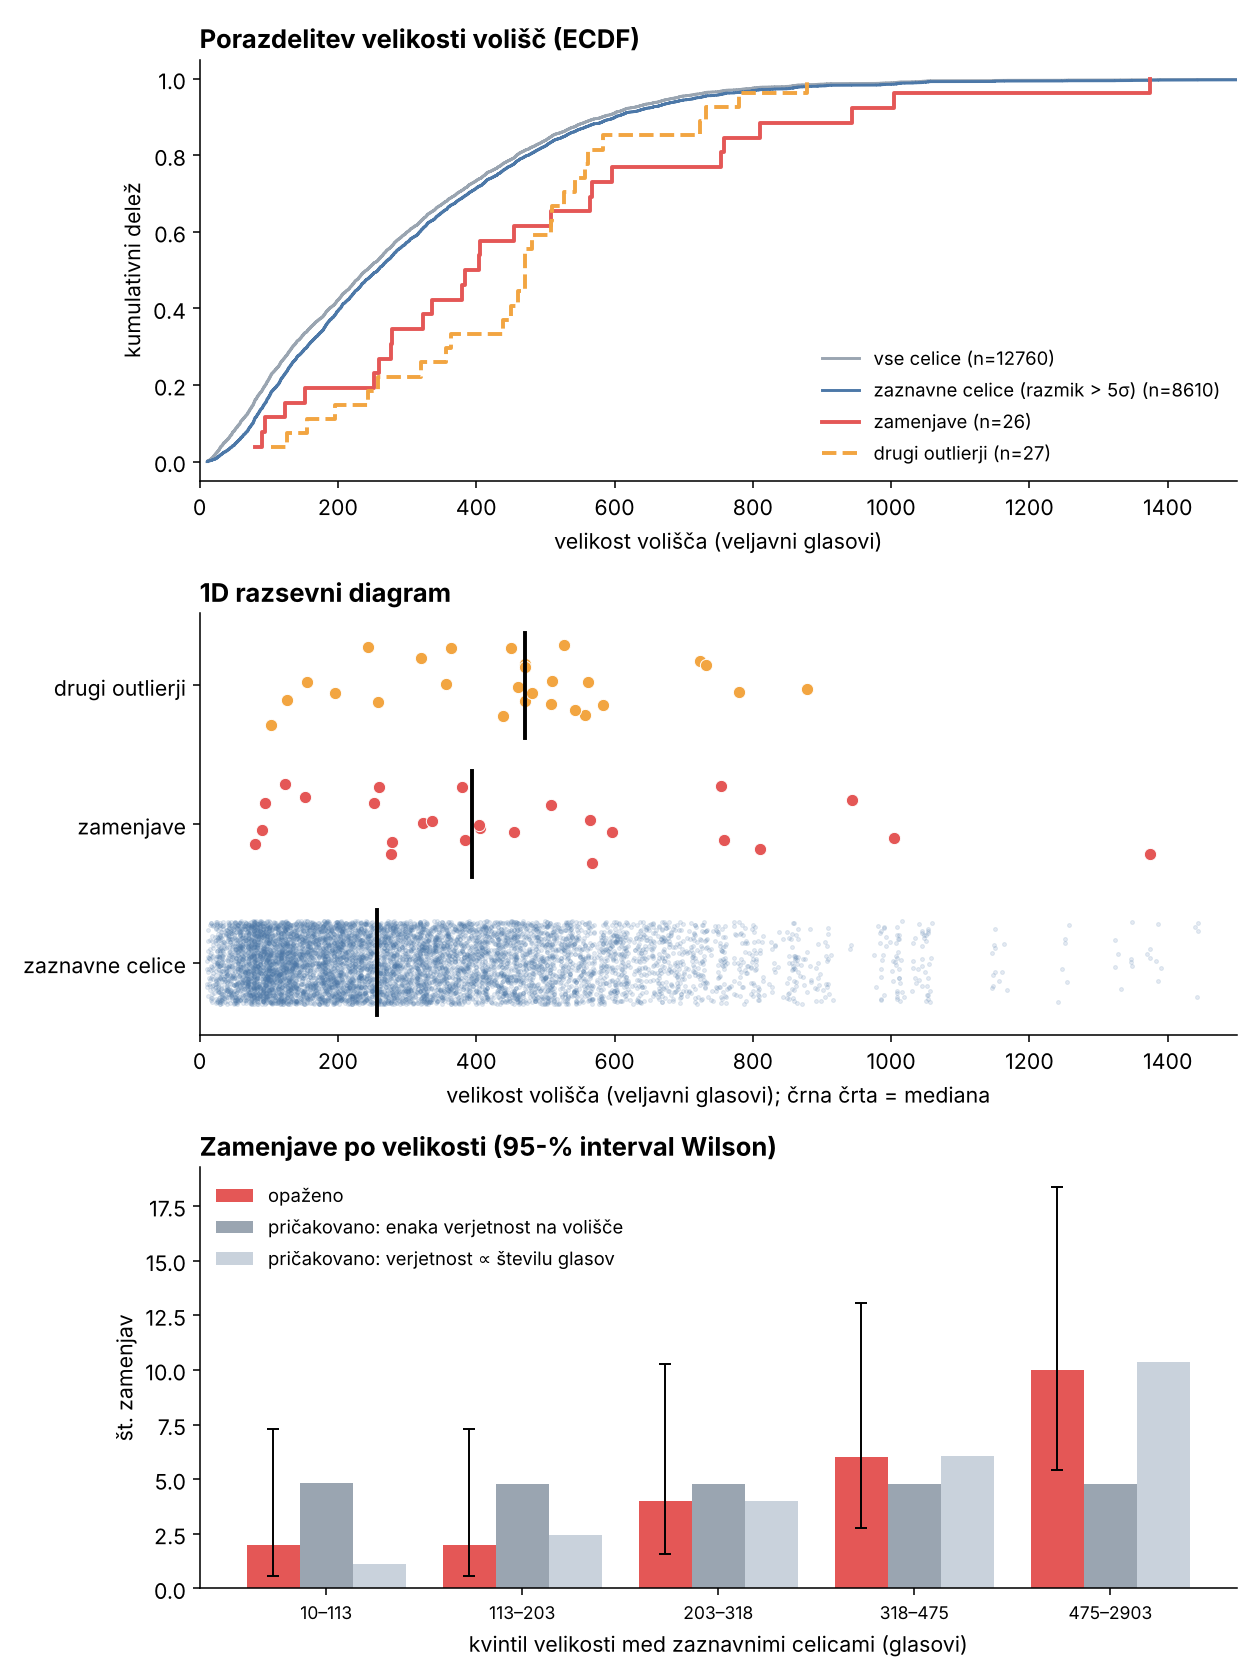
\includegraphics[width=0.75\textwidth]{13_velikost.png}
\caption{Velikost volišč (število veljavnih glasovnic) pri domnevnih zamenjavah v primerjavi z vsemi celicami, kjer bi bila zamenjava zaznavna (razmik $>5\sigma$). Zgoraj: kumulativna porazdelitev velikosti. Sredina: vsaka točka je ena celica, črna črta je mediana. Spodaj: število zamenjav po petinah (kvintilih) velikosti z 95-\% intervalom zaupanja, v primerjavi z dvema hipotezama: enaka verjetnost napake za vsako volišče (temno sivo) ali verjetnost sorazmerna s številom glasov (svetlo sivo). Podatki se ujemajo z drugo hipotezo.}
\label{fig:velikost}
\end{figure}

%=====================================================
\clearpage
\section{Ali gre res za napake?}

Ključno vprašanje je, ali je sum na napake upravičen, ali pa gre pri outlierjih za volišča z resnično (morda zelo ekstremno) posebnostjo, ob kateri napak sploh ni. Kriterij $|z^{\text{zam}}|<3$ sam po sebi ni dokaz: pri volišču z napovedjo blizu 50~\% je zrcalna vrednost blizu objavljene. Spodaj je zato več testov, od enostavnih do takih, ki ne temeljijo na predhodni razvrstitvi (razdelek~\ref{sec:lambda}). Razdelki~4.1--\ref{sec:stavba} uporabljajo razvrstitev med zamenjave in ostale outlierje iz razdelka~\ref{sec:razvrstitev}, razdelka~\ref{sec:zrcalnaos} in~\ref{sec:lambda} pa ne.

\subsection{Diagnostični diagram}

Velja $z - z^{\text{zam}} = (1-2\hat p)/\text{šum}$. Normalna volišča so v pasu $|z|<5$, kjer $z^{\text{zam}}$ niha poljubno; zamenjave so outlierji v vodoravnem pasu $|z^{\text{zam}}|<3$ (slika~\ref{fig:diag}).

\begin{figure}[H]
\centering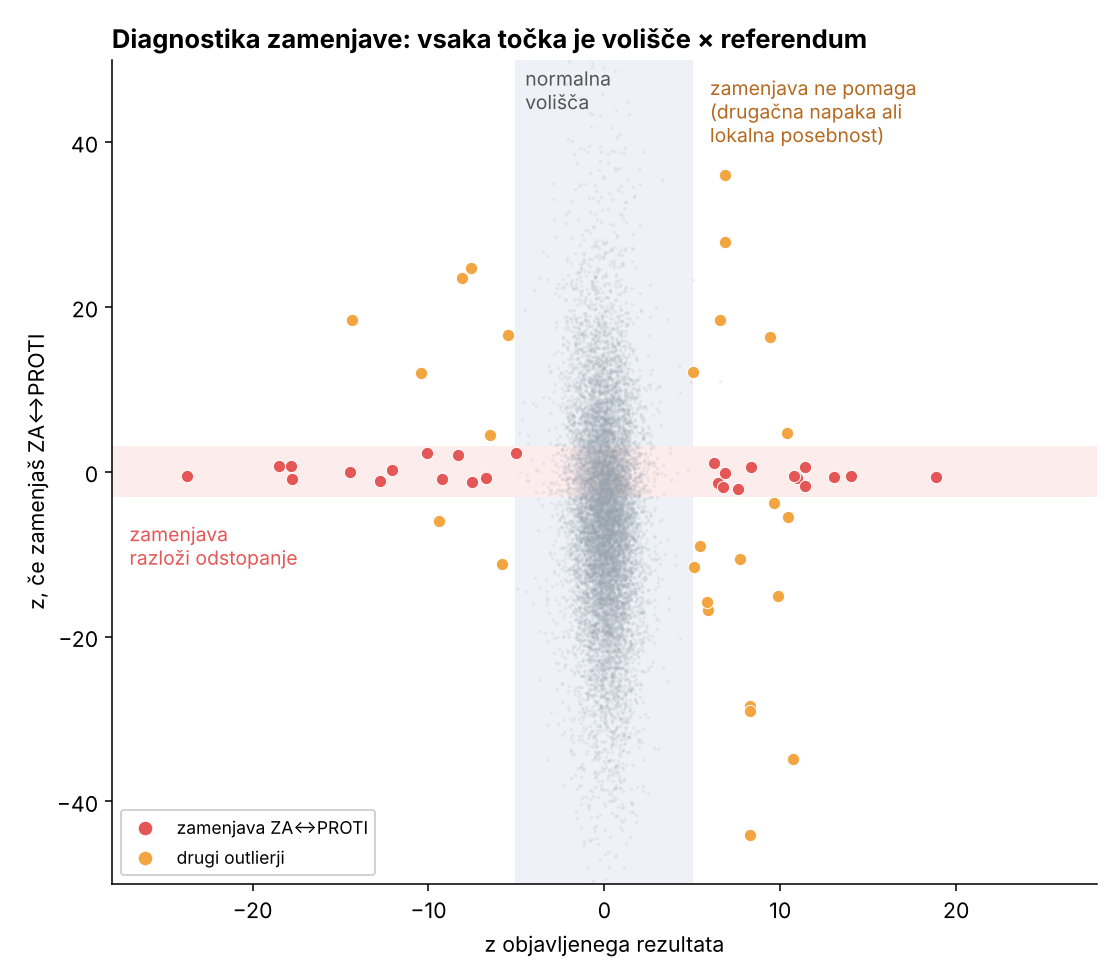
\includegraphics[width=0.7\textwidth]{2_diagnostika_zamenjave.png}
\caption{Diagnostika zamenjave; vsaka točka je celica (volišče $\times$ referendum). Vodoravno: odstopanje objavljenega rezultata od napovedi $z$; navpično: odstopanje, če bi zamenjali ZA in PROTI, $z^{\text{zam}}$. Siv navpični pas: $|z|<5$ (normalne celice). Rdeč vodoravni pas: $|z^{\text{zam}}|<3$; outlier v tem pasu se po zamenjavi ujema z napovedjo (domnevna zamenjava ZA$\leftrightarrow$PROTI, rdeče). Oranžno: outlierji, ki jih zamenjava ne pojasni.}
\label{fig:diag}
\end{figure}

\subsection{Ničelna hipoteza: naključna odstopanja}

\textbf{Metoda.} 400\,000-krat izberem naključno volišče in referendum, njegovemu dejanskemu deležu ZA dodam umetno odstopanje, izračunam $z$ in $z^{\text{zam}}$ z istim modelom, obdržim primere z $|z|>5$ in preštejem, kolikšen delež pade v pas $|z^{\text{zam}}|<3$. Tri različice umetnega odstopanja:

\begin{center}
\begin{tabular}{p{8.5cm}ccc}
\toprule
Ničelna hipoteza & v pasu & pričak. od 53 & $P(\geq27)$ \\
\midrule
A: napake enake velikosti kot pri vseh 53 outlierjih, naključni predznak & 13,8 \% & 7,3 & $2\cdot10^{-8}$ \\
B: resničen lokalni učinek (premik v logitih, Studentova $t_3$) & 14,3 \% & 7,6 & $4\cdot10^{-8}$ \\
C: povsem naključen delež 0--100 \% & 16,2 \% & 8,6 & $4\cdot10^{-7}$ \\
\bottomrule
\end{tabular}
\end{center}

Opaženih je 27.

Hipoteza A uporabi velikosti odstopanj vseh 53 outlierjev, tudi domnevnih zamenjav, zato ni odvisna od razvrstitve; rezultat je praktično enak kot ob uporabi samo outlierjev, ki niso zamenjave (13,9~\%). Hipotezi B in C sta od opaženih outlierjev povsem neodvisni.

\subsection{Razporeditev znotraj pasu}

Če je zamenjava prava, je $1-p$ pravi rezultat volišča in $z^{\text{zam}}\sim N(0,1)$. Naključna odstopanja, ki padejo v pas, pa so v njem razporejena enakomerno.

\begin{center}
\begin{tabular}{lccc}
\toprule
$|z^{\text{zam}}|$ & 0--1 & 1--2 & 2--3 \\
\midrule
Opaženo & \textbf{17} & \textbf{6} & \textbf{4} \\
Vse naključno & 2,5 & 2,4 & 2,4 \\
23 pravih zamenjav $\sim N(0,1)$ + naključno ozadje & 17,1 & 7,6 & 2,4 \\
\bottomrule
\end{tabular}
\end{center}

Model ``23 pravih zamenjav + ozadje'' se z opaženim skoraj popolnoma ujema. Med 27 celicami v pasu je torej verjetno 2--4 lažnih zadetkov, predvsem pri $|z^{\text{zam}}|$ med 2 in 3. V 20\,000 simulacijah ``vse naključno'' ni bilo nikoli 17 ali več točk znotraj $\pm1$ (95. centil: 5). Opažene točke v pasu imajo povprečje $-0{,}23$ in standardni odklon 1,18 (pričakovano 0 in 1).

\begin{figure}[H]
\centering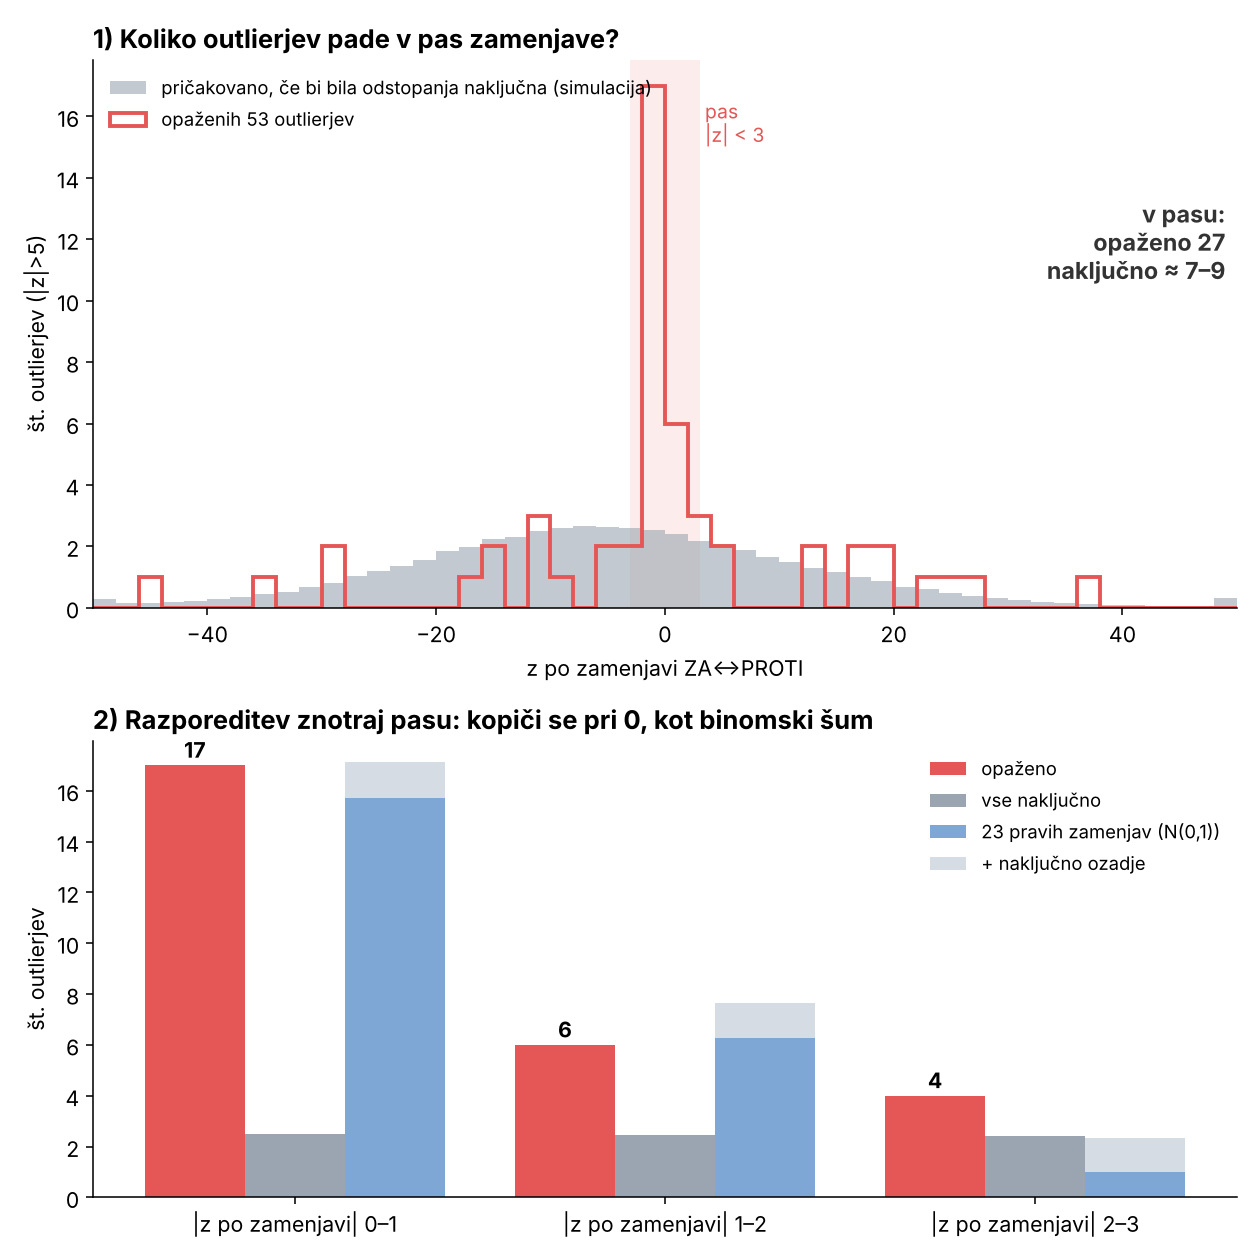
\includegraphics[width=0.8\textwidth]{9_test_pasu.png}
\caption{Zgoraj: porazdelitev $z^{\text{zam}}$ za 53 outlierjev (rdeča črta) v primerjavi s simulacijo, v kateri so odstopanja naključna (sivo, prerazporejeno na 53 outlierjev); rdeč pas je $|z^{\text{zam}}|<3$. Siva porazdelitev ni centrirana pri 0: za outlier, ki ni zamenjava, je $z^{\text{zam}}\approx$ razmik $-\,z$, razmik pa je pri večini celic negativen, ker je pri 67~\% celic napoved nad 50~\% ZA (sociala in tujci sta imela večino ZA); mediana je okoli $-5$. Spodaj: razporeditev outlierjev znotraj pasu $|z^{\text{zam}}|<3$ po razredih (rdeče) v primerjavi s hipotezo ``vse naključno'' (sivo) in s hipotezo ``23 pravih zamenjav, porazdeljenih normalno, plus naključno ozadje'' (modro in svetlo sivo).}
\label{fig:pas}
\end{figure}

\begin{figure}[H]
\centering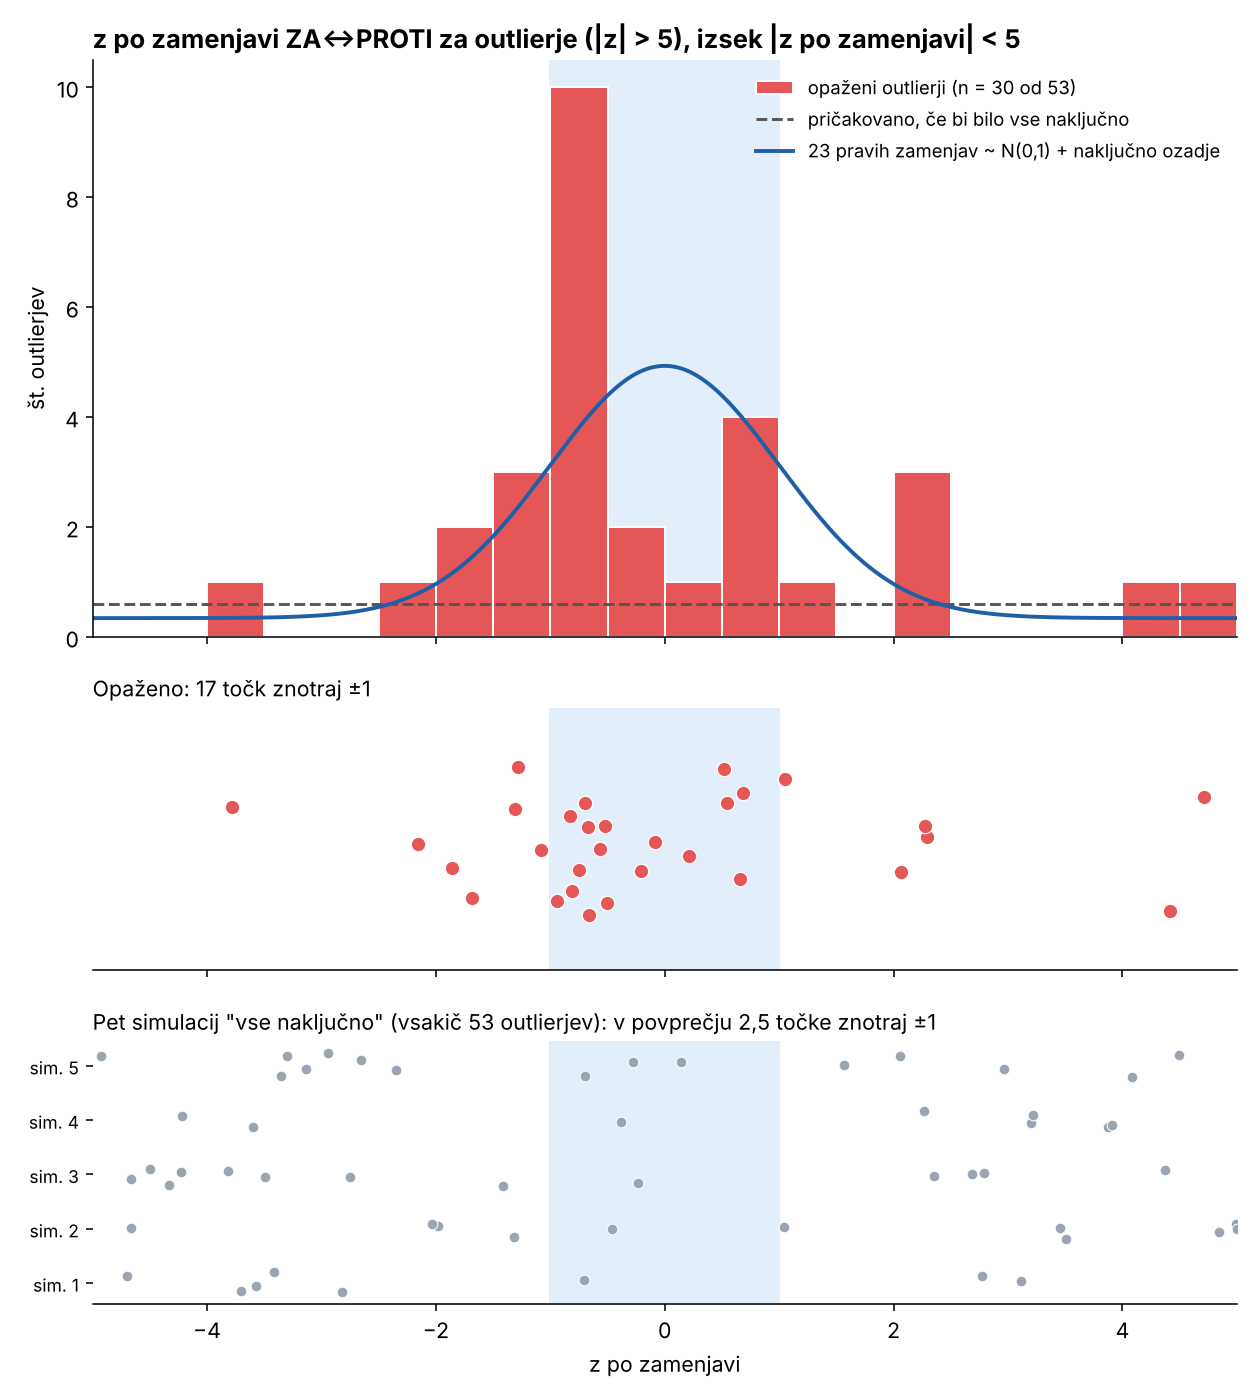
\includegraphics[width=0.75\textwidth]{11_z_po_zamenjavi_zoom.png}
\caption{Izsek $|z^{\text{zam}}|<5$ (30 od 53 outlierjev). Zgoraj: histogram opaženih vrednosti (rdeče), pričakovanje, če bi bila vsa odstopanja naključna (črtkano), in model ``23 pravih zamenjav $\sim N(0,1)$ plus naključno ozadje'' (modra krivulja); modri pas je $|z^{\text{zam}}|<1$. Sredina: vsaka točka je en opažen outlier (navpični razmik je le za preglednost). Spodaj: pet simulacij po 53 outlierjev ob hipotezi ``vse naključno''; v pasu $\pm1$ jih je v povprečju 2,5, opaženih je 17.}
\label{fig:zoom}
\end{figure}

\subsection{Zakaj resnična lokalna posebnost ne pade na zrcalno črto}

Slika~\ref{fig:zrc} kaže iste celice kot slika~\ref{fig:diag}, le v drugih koordinatah. Na sliki~\ref{fig:diag} sta osi neposredno veličini iz pravil za razvrščanje ($z$ in $z^{\text{zam}}$), zato sta outlierji in zamenjave ločeni s pravokotnima pasovoma. Na sliki~\ref{fig:zrc} pa je na vodoravni osi razdalja napovedi od 50~\%, torej premik, ki bi ga povzročila zamenjava, na navpični pa dejanski premik objavljenega rezultata od napovedi, oboje v odstotnih točkah; enak prikaz v enotah šuma čez vse celice je na sliki~\ref{fig:os}. Normalne celice zato ležijo na vodoravni osi, zamenjave pa na diagonali $p-\hat p = 1-2\hat p$. Ta prikaz pokaže, zakaj so zamenjave posebne: dejanski premik je pri vsaki od njih točno tolikšen, kot ga zahteva zrcaljenje.

Resnična posebnost volišča (sestava volivcev, lokalna tema, zmeda pri vprašanju) premakne rezultat za količino, ki ni povezana z oddaljenostjo napovedi od 50~\%. Da bi resničen premik padel na zrcalno črto, bi moral biti naključno natanko dvakratna razdalja napovedi od 50~\% (pri napovedi 36~\% točno $+28$ točk), oziroma bi moral vsak volivec glasovati nasprotno od svojega namena. Takšni premiki se razpršijo po ravnini, kot oranžne točke na sliki; rdeče se nanizajo na črto v obeh smereh in pri različnih razdaljah od 50~\%. To je podpis mehanske operacije s števili (dve števili zamenjata mesti). V logitih zrcaljenje pomeni premik točno $-2\operatorname{logit}\hat p$, pri napovedi 36~\% torej $+1{,}15$, pri 70~\% pa $-1{,}7$: resnična posebnost bi morala na vsakem volišču zadeti drugo vrednost do natančnosti šuma. Prikaz pokaže tudi, zakaj zamenjav blizu 50~\% ni mogoče zaznati: tam se diagonala in vodoravna os stikata.

\begin{figure}[H]
\centering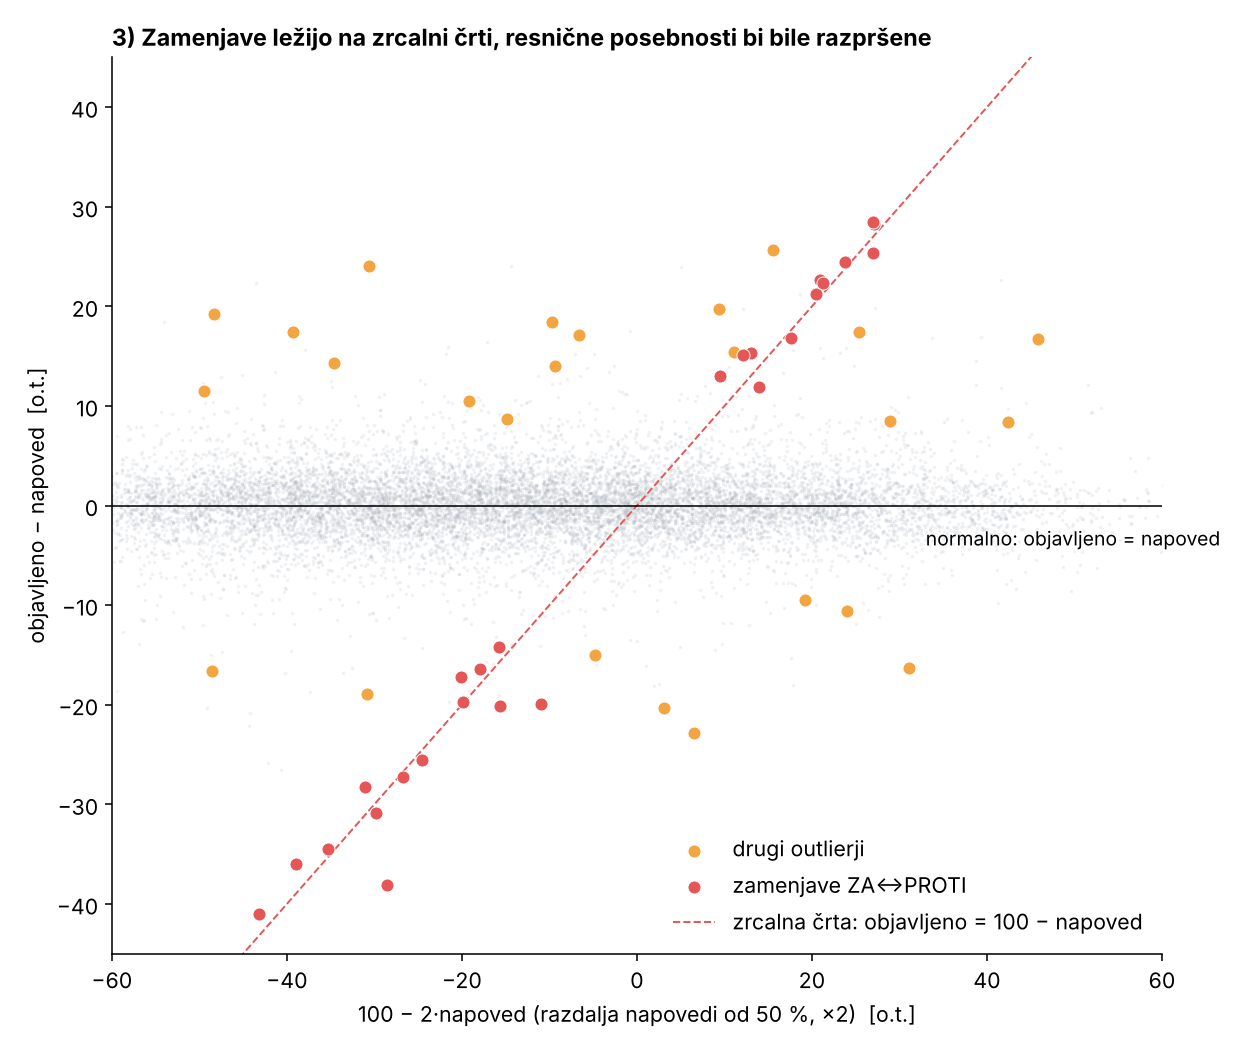
\includegraphics[width=0.75\textwidth]{10_zrcalna_crta.png}
\caption{Vsaka točka je celica. Navpično: objavljeni delež minus napoved; vodoravno: $100-2\cdot$napoved, torej koliko bi se rezultat spremenil, če bi zamenjali ZA in PROTI (v odstotnih točkah). Normalne celice ležijo na vodoravni osi (siva megla), celice z zamenjanima ZA in PROTI pa na rdeči črtkani diagonali. Rdeče: domnevne zamenjave ZA$\leftrightarrow$PROTI; oranžno: drugi outlierji, ki so razpršeni po ravnini, kot bi pričakovali pri resničnih posebnostih.}
\label{fig:zrc}
\end{figure}

\subsection{Volišča v isti stavbi}\label{sec:stavba}

Volivci v isti stavbi so si demografsko zelo podobni, zato bi se resnična posebnost pokazala tudi pri sosednjih voliščih. Pri osmih domnevnih zamenjavah ZA$\leftrightarrow$PROTI so v isti stavbi še druga volišča (iskano po imenu stavbe in naslovu). Pri sedmih od njih je objavljeni rezultat od sosednjih volišč oddaljen 15--39 odstotnih točk, rezultat po zamenjavi pa le 0--7 točk:

\begin{center}
\small\begin{tabular}{llrrrl}
\toprule
 & & \multicolumn{4}{c}{delež ZA (\%)} \\
\cmidrule(lr){3-6}
Volišče z domnevno zamenjavo & referendum & objavljeno & po zamenjavi & napoved & sestrska volišča \\
\midrule
Koper~1/22, SEPŠ & preiskava & \textbf{65} & 35 & 36 & 32, 30, 31, 31, 36 \\
Moste-Polje~3/18, Kodeljevo & preiskava & \textbf{65} & 35 & 37 & 37, 31, 34 \\
Vič-Rudnik~4/31, Obrtna zbornica & RTV & \textbf{62} & 38 & 40 & 45 \\
Logatec/30, OŠ 8 talcev & sociala & \textbf{40} & 60 & 60 & 55 \\
Ptuj~2/24, DK Turnišče & sociala & \textbf{31} & 69 & 72 & 69 \\
Žalec~2/37, Dom kulture Braslovče & sociala & \textbf{34} & 66 & 65 & 68 \\
Brežice/8, SIC Brežice & RTV & \textbf{62} & 38 & 37 & 45 \\
Moste-Polje~1/24, OŠ Sostro & preiskava & \textbf{58} & 42 & 45 & 46, 55 \\
\bottomrule
\end{tabular}
\end{center}

Pri prvih sedmih so sestrska volišča pri istem referendumu povsem v skladu z napovedjo ($|z|\leq1{,}7$ pri vseh). Izjema je OŠ Sostro: volišče~21 se ujema z zamenjavo (46~\%), volišče~25 pa ima pri preiskavi podoben rezultat kot domnevna zamenjava (55~\%, $z=+10$). Tam podatki ne ločijo med zamenjavo in lokalno posebnostjo; tudi mešani model temu primeru pripiše le okoli 0,5 verjetnosti za zamenjavo.

\subsection{Zgoščevanje ob zrcalni osi čez vse podatke}\label{sec:zrcalnaos}

Zrcalno os sem podaljšal čez vseh 12\,760 celic in jih razvrstil po razmiku med normalo in zrcalno osjo, $(1-2\hat p)/\text{šum}$. V vsakem razredu sem preštel celice v pasu $|z^{\text{zam}}|<1$ in jih primerjal s pričakovanjem, če odstopanje celice ni povezano z njenim razmikom. Za pričakovanje uporabim empirično porazdelitev $z$ vseh 12\,760 celic, brez izločanja zamenjav ali drugih outlierjev, zato vsebuje dejanske debele repe in izračun ni krožen. Celica z razmikom $s$ leži ob zrcalni osi, če njen $z$ pade v interval $[s-1,\,s+1]$; verjetnost za to je delež vseh celic, katerih $z$ leži v tem intervalu, pričakovano število v razredu pa vsota teh verjetnosti po celicah razreda. Negotovost presežka je binomski standardni odklon ob ničelni hipotezi.

\begin{center}
\begin{tabular}{lrrrr}
\toprule
razmik [$\sigma$] & celic & opaženo & pričakovano & presežek \\
\midrule
0--1 & 857 & 553 & 518,9 & $+34\pm14$ \\
1--2 & 863 & 265 & 264,2 & $+1\pm13$ \\
2--3 & 833 & 77 & 63,3 & $+14\pm8$ \\
3--4 & 790 & 15 & 9,5 & $+5\pm3$ \\
4--6 & 1450 & 4 & 2,2 & $+2\pm1{,}5$ \\
6--10 & 2553 & 5 & 1,5 & $+3{,}5\pm1{,}2$ \\
10--20 & 3682 & 11 & 0,7 & $+10{,}3\pm0{,}8$ \\
20--60 & 1701 & 1 & 0,0 & $+1$ \\
\bottomrule
\end{tabular}
\end{center}

Nad $4\sigma$ je presežek jasen (21 proti 4,4; Poisson $p\approx10^{-8}$). To je konzervativno, saj pričakovanje vključuje tudi same zamenjave, ki rep porazdelitve $z$ odebelijo. Pri razmiku 2--4$\sigma$ je presežek okoli $19\pm8$ (približno $2{,}3\sigma$), kar nakazuje dodatne zamenjave pri voliščih z napovedjo blizu 50~\%, ki ne dosežejo praga $|z|>5$ in jih posamično ni mogoče identificirati. Presežek pri razmiku pod $1\sigma$ ($34\pm14$) je treba razlagati previdno: tam se pas ob zrcalni osi skoraj prekriva z normalo, zato je odvisen od natančne oblike jedra porazdelitve $z$. Oceno skupnega števila zamenjav, vključno z nezaznavnimi, podajam v razdelku~\ref{sec:skupno}; zamenjave blizu 50~\% so nevidne, a tudi brez vpliva.

\begin{figure}[H]
\centering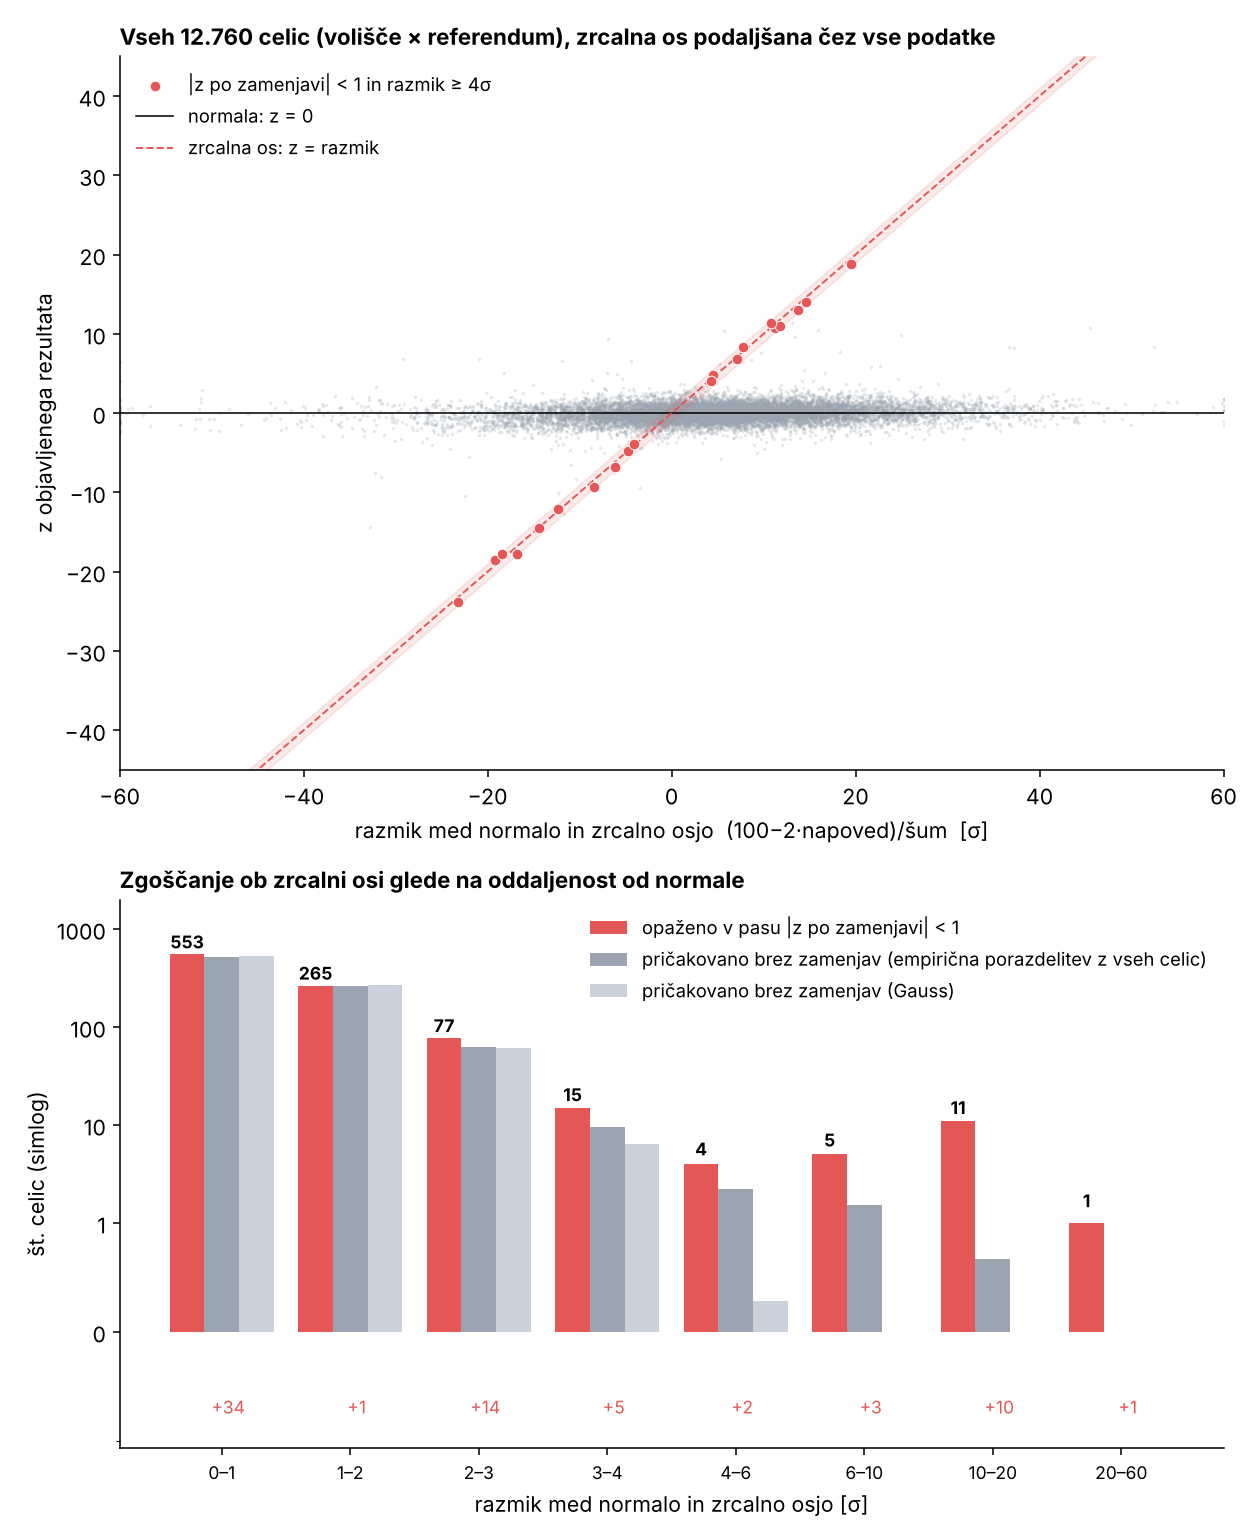
\includegraphics[width=0.75\textwidth]{12_zrcalna_os_vsi.png}
\caption{Zgoraj: vseh 12\,760 celic; vodoravno razmik (oddaljenost napovedi od 50~\% v enotah šuma), navpično $z$. Normala ($z=0$) je vodoravna, zrcalna os ($z=$ razmik) je diagonala z rdečim pasom $\pm1$. Rdeče so celice, ki ležijo ob zrcalni osi pri razmiku vsaj $4\sigma$. Spodaj: za vsak razred razmika opaženo število celic v pasu $|z^{\text{zam}}|<1$ (rdeče) in pričakovano število brez zamenjav iz empirične porazdelitve $z$ vseh celic (temno sivo) oziroma normalne porazdelitve (svetlo sivo); rdeče številke spodaj so presežki. Navpična os je logaritemska.}
\label{fig:os}
\end{figure}

\subsection{Analiza vseh outlierjev brez izbire širine pasu zamenjav}
\label{sec:lambda}

Testi v razdelkih~4.2--\ref{sec:stavba} uporabljajo pas zamenjav $|z^{\text{zam}}|<3$, katerega širina je izbrana. Tu pasu ne uporabim: vzamem vseh 53 outlierjev, izbranih \emph{samo} po $|z|>5$, in za vsakega izračunam njegov položaj na premici od normale do zrcalne osi,
\begin{equation}
\lambda = \frac{p-\hat p}{1-2\hat p},\qquad \sigma_\lambda = \frac{\text{šum}}{|1-2\hat p|},
\label{eq:lambda}
\end{equation}
kjer $\lambda=0$ pomeni rezultat kot napoved in $\lambda=1$ popolno zamenjavo ZA$\leftrightarrow$PROTI.

\textbf{Ničelne hipoteze brez napak.} Simuliral sem štiri mehanizme brez zamenjav, vsakič z istim izborom $|z|>5$: resnično lokalno posebnost (premik v logitih, $t_3$), povsem naključen delež, del glasovnic preštet v napačni kup (naključen delež $f\in(0,1)$ ene strani) in napako v enem samem številu (ZA ali PROTI pomnoženo z naključnim faktorjem). Nobeden ne ustvari vrha pri $\lambda=1$; vsi dajo široko gladko porazdelitev (slika~\ref{fig:lambda}). Opaženih je 17 outlierjev z $\lambda\in[0{,}9;\,1{,}1]$, pričakovano 2,4--3,7.

\begin{figure}[H]
\centering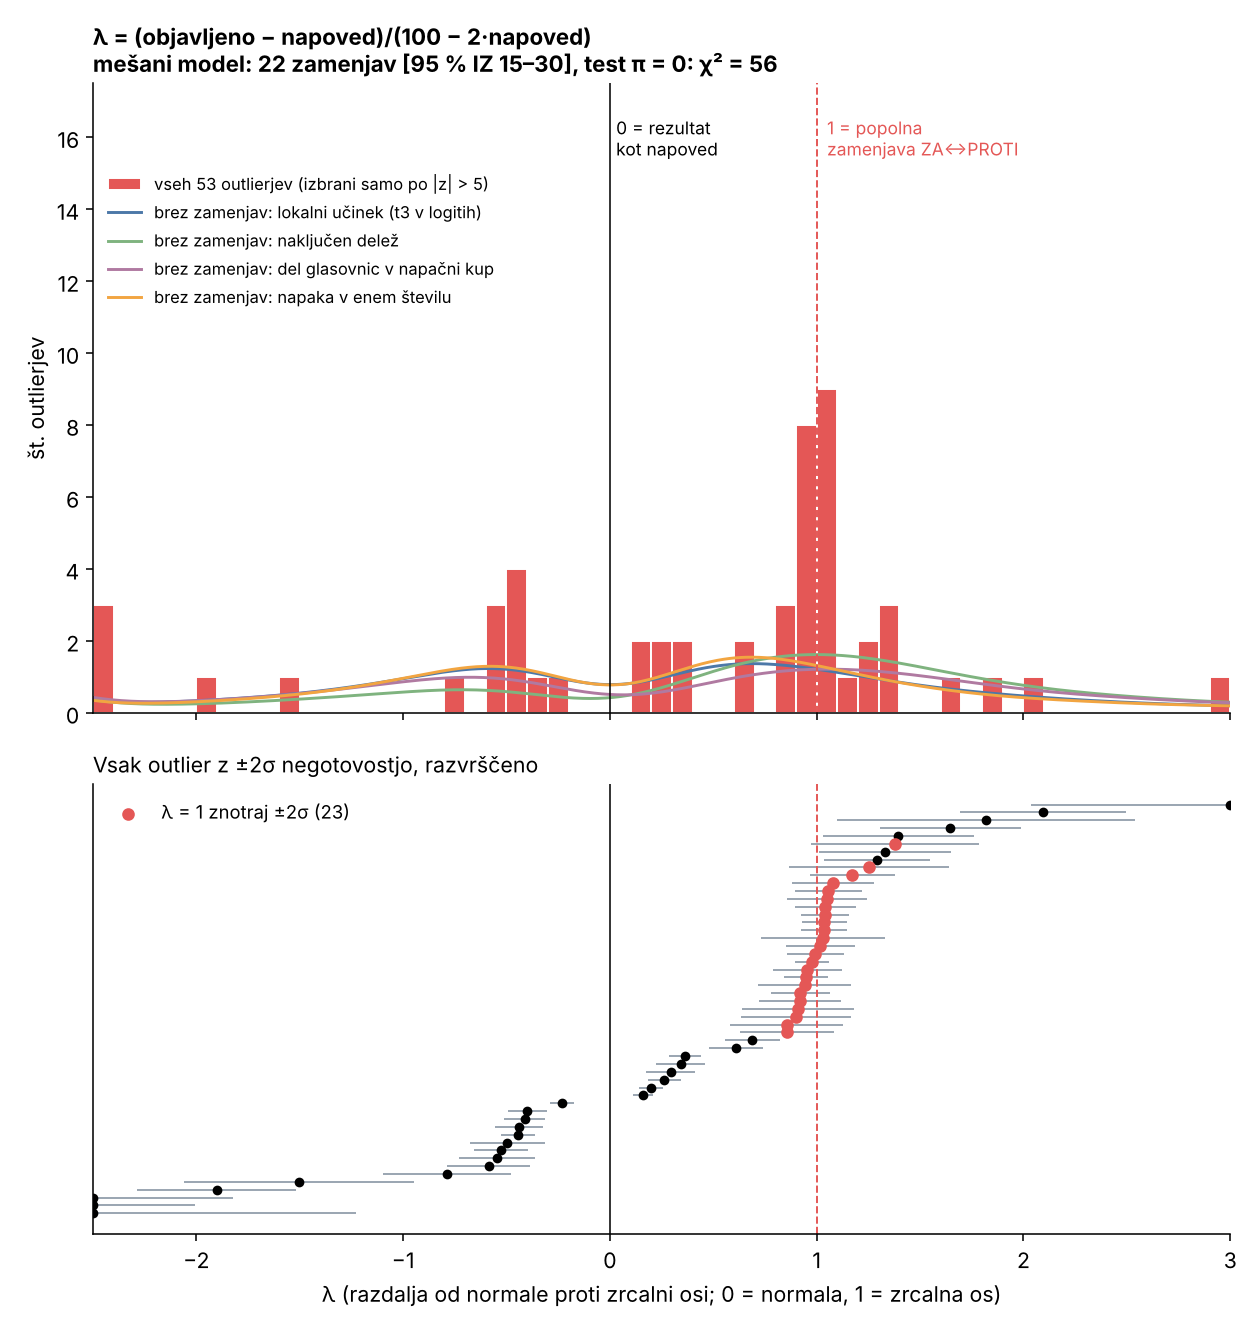
\includegraphics[width=0.8\textwidth]{14_lambda_mesanica.png}
\caption{Zgoraj: porazdelitev $\lambda$ za vseh 53 outlierjev, izbranih samo po $|z|>5$ (rdeči stolpci); $\lambda=0$ pomeni rezultat kot napoved, $\lambda=1$ popolno zamenjavo ZA$\leftrightarrow$PROTI. Barvne krivulje so pričakovane porazdelitve, če zamenjav ne bi bilo, pri štirih različnih mehanizmih (ozadjih); nobena nima vrha pri $\lambda=1$. Spodaj: vsak outlier posebej z negotovostjo $\pm2\sigma_\lambda$ (vodoravna črta), urejeno po $\lambda$; rdeči so tisti, pri katerih je $\lambda=1$ znotraj negotovosti.}
\label{fig:lambda}
\end{figure}

\textbf{Mešani model.} Naj bo $\pi$ delež outlierjev, ki so zamenjave ZA$\leftrightarrow$PROTI (preostalih $1-\pi$ so outlierji drugega izvora). Verjetje outlierja je $\pi\,N(1,\sigma_{\lambda,i}) + (1-\pi)\,h(\lambda_i)$, kjer je $h$ porazdelitev $\lambda$ iz simulacije brez zamenjav. To porazdelitev v nadaljevanju imenujem \emph{ozadje}: je porazdelitev $\lambda$ pri ničelni hipotezi (brez zamenjav), ob alternativi pa opisuje outlierje, ki niso zamenjave. Ničelna hipoteza je $\pi=0$. $\pi$ ocenim z največjim verjetjem, interval zaupanja s profilnim verjetjem. Ničelno hipotezo preverim s testom razmerja verjetij, $\chi^2=2[\ell(\hat\pi)-\ell(0)]$, z 1 prostostno stopnjo; ker $\pi=0$ leži na robu dovoljenega območja, je $p=P(Z>\sqrt{\chi^2})$ za standardno normalno $Z$.

\begin{center}
\begin{tabular}{lcccc}
\toprule
Ozadje (ničelna porazdelitev) & $\pi$ & št. zamenjav [95-\% IZ] & $\chi^2$ (1 s.p.) & $p$ \\
\midrule
resnična lokalna posebnost & 0,42 & 22 [15--30] & $56$ & $<10^{-10}$ \\
naključen delež & 0,39 & 21 [13--29] & $42$ & $<10^{-10}$ \\
del glasovnic v napačnem kupu & 0,41 & 22 [14--30] & $53$ & $<10^{-10}$ \\
napaka v enem številu & 0,42 & 22 [14--30] & $53$ & $<10^{-10}$ \\
\bottomrule
\end{tabular}
\end{center}

Izračunane $p$-vrednosti so reda $10^{-11}$ do $10^{-14}$, vendar jih ne gre jemati dobesedno: izračun je asimptotski, ozadje je ocenjeno iz simulacije in komponenta zamenjav ima predpostavljeno obliko. Pri tako majhnih vrednostih napačna specifikacija modela prevlada nad statistično negotovostjo, zato navajam le zgornjo mejo $p<10^{-10}$. Ocena je robustna na izbiro ozadja in se ujema s 26 ročno označenimi zamenjavami, zmanjšanimi za ocenjene 2--4 lažne zadetke.

\textbf{Robustnost na velikost volišča.} Zamenjave so na večjih voliščih (razdelek~\ref{sec:velikost}). Če bi bile tudi nedolžne posebnosti iz neznanega razloga povezane z velikostjo, bi to lahko vplivalo na ozadje. Zato sem analizo ponovil z dvema strožjima ničelnima modeloma:
\begin{itemize}
\item \emph{Ujemanje velikosti}: simulirane posebnosti so prevrednotene tako, da imajo enako porazdelitev velikosti volišč kot opaženi outlierji. Ocena ostane 21--23 zamenjav [13--31], $p<10^{-10}$.
\item \emph{Ista volišča}: najstrožja različica. Obdržim točno istih 53 celic (iste velikosti in napovedi) in jim namesto opaženega rezultata pripišem naključno resnično posebnost, ki da $|z|>5$. Pričakovano število v jedru $\lambda\in[0{,}9;\,1{,}1]$ je 2,9--3,8, opaženih 17 ($P\approx10^{-9}$).
\end{itemize}
Velikost volišča vpliva le na širino porazdelitve $\lambda$ (večje volišče ima manjši šum in ožji pas okoli zrcalne osi), ne more pa ustvariti vrha na zrcalni vrednosti, ki je za vsako volišče drugačna.

\textbf{Test gladkosti brez modela ozadja.} Katera koli resnična posebnost, ne glede na to, kako ekstremna ali debelorepa je, da gladko porazdelitev $\lambda$, ker je $\lambda$ zvezna funkcija velikosti posebnosti in napovedi, napovedi pa se med volišči razlikujejo. Edina predpostavka je, da velikost posebnosti ni ``uglašena'' točno na zrcalno vrednost. V jedru $\lambda\in[0{,}9;\,1{,}1]$ je 17 outlierjev, v sosednjih pasovih štirikrat večje skupne širine (0,5--0,9 in 1,1--1,5) pa 11; gladko ozadje bi v jedro postavilo 2,8 (binomski test $p\approx3\cdot10^{-6}$). Pri ožjem jedru $\pm0{,}05$: 9 proti 3,0 ($p\approx0{,}014$).

\subsection{Ocena skupnega števila zamenjav}\label{sec:skupno}

Zamenjavo je mogoče zaznati le, če je volišče dovolj daleč od 50:50. Za vsako od 12\,760 celic sem izračunal verjetnost, da bi zamenjava dala $|z|>5$ v obeh modelih (odvisna je le od razmika med normalo in zrcalno osjo); povprečno je 0,67 (uteženo s številom glasov 0,71), pri tretjini celic je pod 0,5. Če ocenjeno število zaznanih zamenjav (okoli 22) delim s to verjetnostjo, dobim okoli 31--33 zamenjav skupaj (95-\% IZ okoli 21--45), torej okoli 0,2--0,3~\% vnosov oziroma okoli 9 na milijon glasov. Ob neodvisnih napakah ima okoli 1~\% volišč zamenjavo pri vsaj enem od štirih referendumov; na en referendum to pomeni okoli 8 zamenjav. To je istega reda velikosti kot pri reviziji novozelandskih volitev 2023 (okoli 0,3--0,7~\% volišč z napako pri vnosu~\cite{oagnz2024}), vendar je primerjava zaradi različnih vrst napak in načinov odkrivanja le okvirna. Ocena velja le za zamenjave ZA$\leftrightarrow$PROTI in predpostavlja, da je verjetnost zamenjave enaka ne glede na oddaljenost od 50:50, kar ni preverljivo. Presežek ob zrcalni osi pri razmiku 2--4$\sigma$ (razdelek~\ref{sec:zrcalnaos}; okoli $19\pm8$ proti okoli 3, ki jih napoveduje ta ocena) nakazuje, da jih je blizu 50:50 morda več, vendar je ta razlika negotova (približno $2\sigma$). Oceno je zato treba razumeti kot spodnjo oceno.

\subsection{Druge kontrole}
\begin{itemize}
\item \textbf{Napaka ni pri branju podatkov}: odstotki v izvorni datoteki se pri vseh 26 zamenjavah ujemajo z (zamenjanimi) števili glasov.
\item \textbf{Ni zgoščenosti po okrajih}: zamenjave so na 21 od 88 okrajev; največ 3 v enem okraju je skladno z naključjem ($p=0{,}31$).
\item \textbf{Porazdelitev po referendumih}: pri sociali je zamenjav nekaj več (11 proti 4--7 pri ostalih). Del razlike pojasni zaznavnost: sociala je imela izrazitejše rezultate (60,5~\% ZA), zato je povprečna verjetnost zaznave zamenjave tam 0,74, pri ostalih 0,58--0,68 (najmanj pri RTV, ki je bil najbližje 50~\%). Ob enaki dejanski stopnji napak bi pričakovali okoli 7,2 zaznane zamenjave pri sociali, 6,6 pri preiskavi, 5,6 pri RTV in 6,6 pri tujcih; preostala razlika je v okviru naključnih nihanj.
\item \textbf{Primerjava enega referenduma z okrajem ne zadošča}: posamična primerjava z mediano okraja ima razpršenost skoraj trikrat večjo od binomske ($c\approx2{,}7$--$3{,}0$), označi predvsem predčasna glasovanja (ki odstopajo pri vseh štirih referendumih hkrati, kar je resničen učinek populacije) in najde le 3 od 26 domnevnih zamenjav ZA$\leftrightarrow$PROTI.
\end{itemize}

\subsection{Sklep}

Tudi če bi presežek outlierjev v celoti pripisali resničnim lokalnim posebnostim ali porazdelitvi, drugačni od predpostavljene, to ne pojasni zgoščevanja na zrcalni vrednosti; to je osrednja ugotovitev analize. Za posamezno volišče to ni dokaz (tega da le zapisnik ali uradni rezultat). Za obstoj napak kot pojava pa daje močno statistično podporo: alternativa bi zahtevala mehanizem resnične posebnosti, ki da rezultat točno na zrcalni vrednosti napovedi na okoli 20 voliščih z različnimi napovedmi, prizadene le enega od štirih referendumov in se ne pokaže v sosednjih voliščih v isti stavbi. Odprto ostaja manjše zgoščenje 8 outlierjev pri $\lambda\approx-0{,}5$, za katerega ne poznam mehanizma; lahko je naključje.

%=====================================================
\section{Vpliv na rezultate}

\begin{center}
\small\begin{tabular}{lrrrrr}
\toprule
 & objavljena & \multicolumn{2}{c}{samo zamenjave} & \multicolumn{2}{c}{vse napake (ocena)} \\
\cmidrule(lr){3-4}\cmidrule(lr){5-6}
Referendum (zmagovalec) & prednost & prednost & sprememba & prednost & sprememba \\
\midrule
Preiskava (PROTI) & 23\,147 & 23\,409 & $+262$ & 23\,782 & $+635$ \\
RTV (PROTI) & 546 & 1\,372 & $+826$ & 1\,320 & $+774$ \\
Sociala (ZA) & 194\,705 & 195\,289 & $+584$ & 195\,225 & $+520$ \\
Tujci (ZA) & 97\,776 & 98\,466 & $+690$ & 97\,771 & $-5$ \\
\bottomrule
\end{tabular}
\end{center}

``Samo zamenjave'': ZA in PROTI zamenjana na 26 celicah. ``Vse napake'': dodatno je pri ostalih outlierjih delež ZA nadomeščen z napovedjo modela (groba ocena, saj so nekateri od teh primerov lahko resnični). Izid se pri nobenem referendumu ne spremeni; delež ZA se premakne za največ 0,04 odstotne točke. Pri RTV, kjer je razlika tesna, bi popravek prednost PROTI povečal približno za dva- do dvainpolkrat (slika~\ref{fig:vpliv}).

\begin{figure}[H]
\centering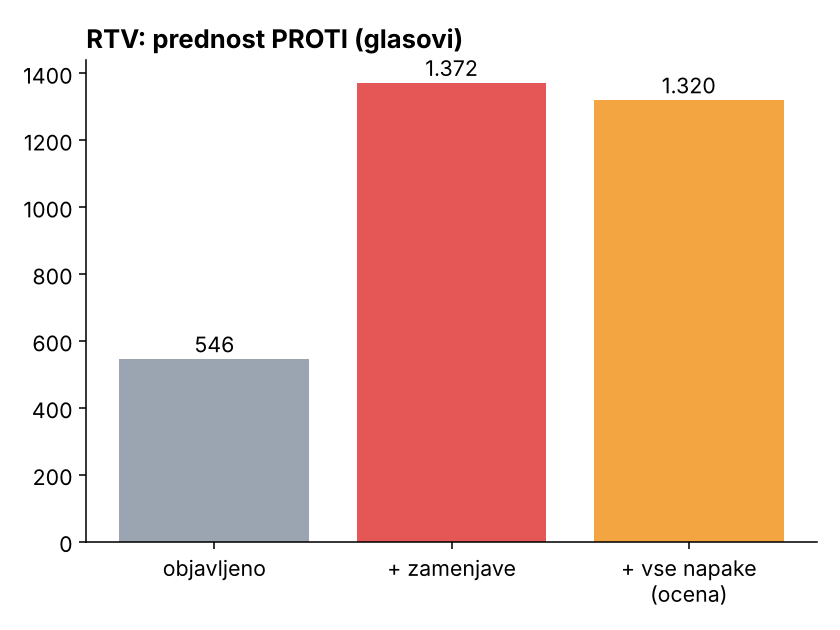
\includegraphics[width=0.5\textwidth]{5_vpliv.png}
\caption{Prednost PROTI na referendumu o RTV v glasovih: objavljena (sivo), po popravku domnevnih zamenjav (rdeče) in po dodatnem popravku ostalih outlierjev z napovedjo modela (oranžno, groba ocena). RTV je edini referendum, kjer je relativni učinek popravkov opazen; za ostale glej tabelo zgoraj.}
\label{fig:vpliv}
\end{figure}


\subsection{Prispevki posameznih volišč (ilustracija)}

Slika~\ref{fig:prispevki} prikazuje, kako bi popravek vsakega volišča z označeno zamenjavo spremenil prednost zmagovalca. Ta prikaz je \textbf{pogojen na hipotezo}, da so označena volišča res zamenjave; za morebitne lažne zadetke popravka ni.

\begin{figure}[H]
\centering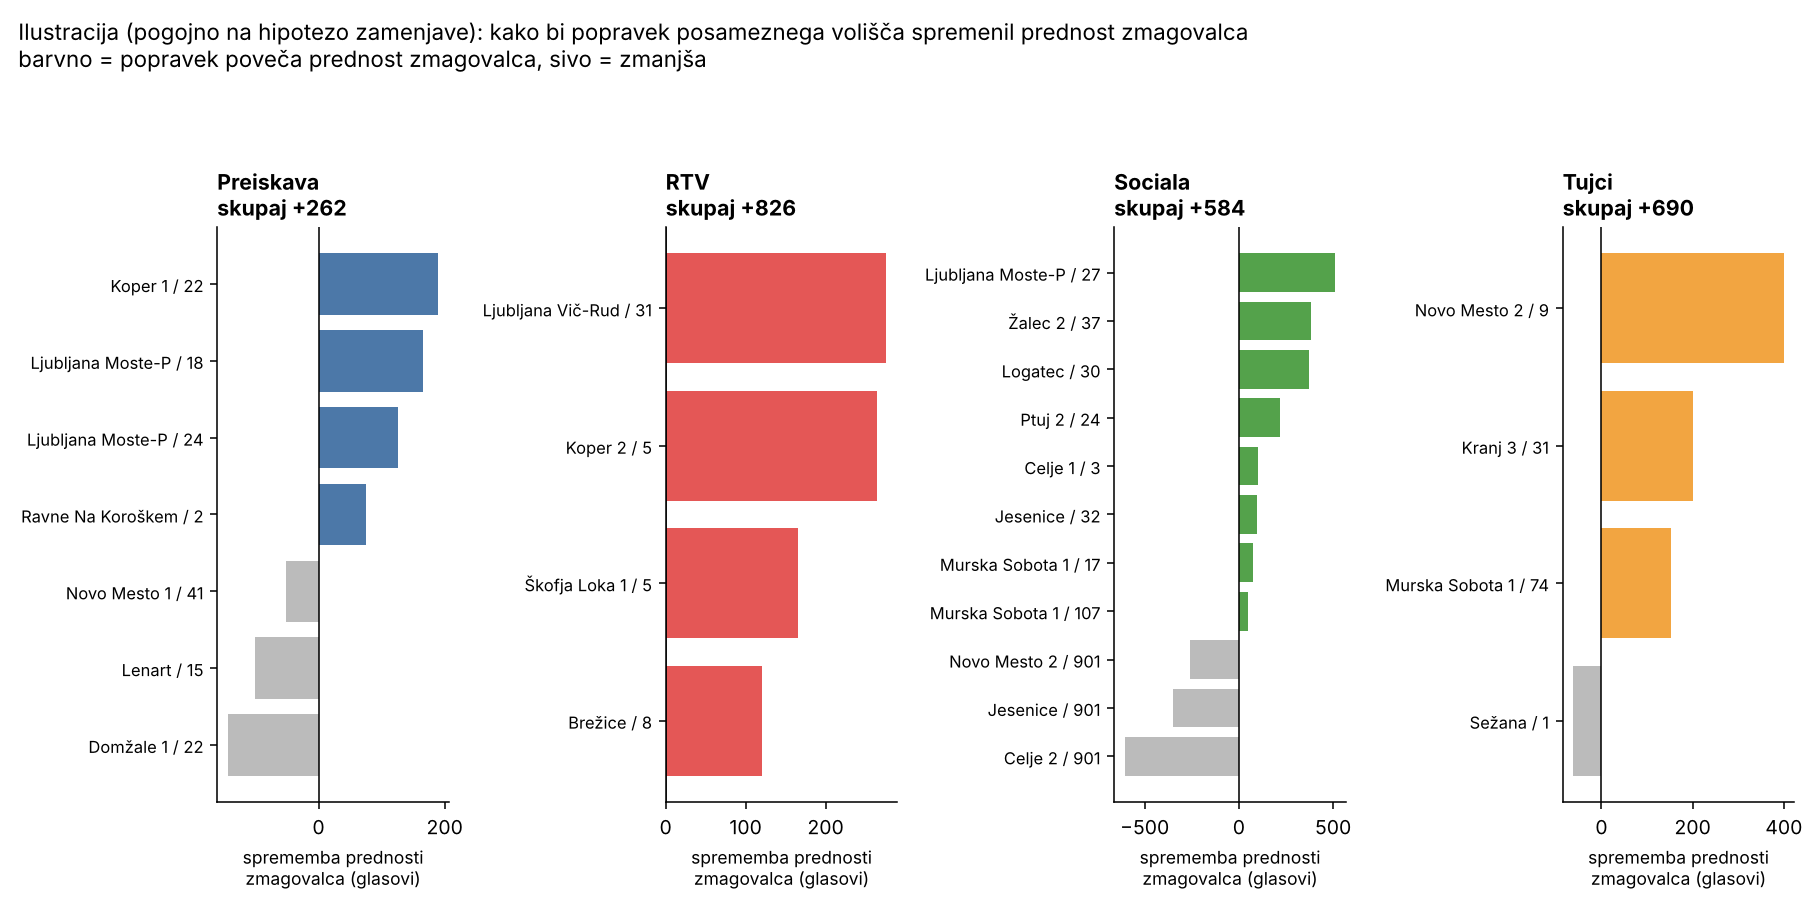
\includegraphics[width=\textwidth]{16_prispevki_volisc.png}
\caption{Za vsako volišče z domnevno zamenjavo ZA$\leftrightarrow$PROTI: za koliko glasov bi se spremenila prednost zmagovalca referenduma, če bi na tem volišču vpisali zamenjana števila. Barvno: popravek poveča prednost zmagovalca; sivo: zmanjša. V naslovu vsakega panela je skupna sprememba. Prikaz je pogojen na to, da so označena volišča res zamenjave.}
\label{fig:prispevki}
\end{figure}

\subsection{Smer napak}
\label{sec:smer}

Pri vseh štirih referendumih popravek označenih zamenjav \emph{poveča} prednost zmagovalca. Pomembno je razumeti, kaj to (ne) pove.

\textbf{Mehanizem.} Zamenjava ZA$\leftrightarrow$PROTI na volišču $i$ z $n_i$ glasovi, kjer ima zmagovalec delež $w_i$, spremeni prednost zmagovalca za $-2(2w_i-1)\,n_i$: glasovi se premaknejo z lokalne večine na lokalno manjšino. Utežena vsota lokalnih prednosti je enaka nacionalni prednosti zmagovalca,
\begin{equation}
\sum_i (2w_i-1)\,n_i = M > 0 .
\label{eq:vsota}
\end{equation}
Če zamenjava zadene naključno volišče (z verjetnostjo, neodvisno od rezultata volišča), je pričakovana sprememba prednosti $-2M/N_{\text{volišč}}<0$ ne glede na to, na koliko voliščih ima zmagovalec večino. Pri preiskavi ima zmagovalec (PROTI) večino le na 44~\% zaznavnih volišč, pa velja enako, ker so ta volišča bistveno večja (povprečno 367 proti 230 glasov). Zamenjave izid v pričakovanju ``stisnejo'' proti 50~\%.

\textbf{Pogojna analiza (le za označene zamenjave).} Za vsak referendum sem z Monte Carlo simulacijo (200\,000 ponovitev) naključno izbral toliko zaznavnih volišč, kolikor je označenih zamenjav, in izračunal spremembo prednosti po popravku.

\begin{center}
\small\begin{tabular}{lcccr}
\toprule
Referendum & zamenjav & v škodo zmag. & sprememba prednosti & pričakovano [95-\% int.] \\
\midrule
Preiskava & 7 & 4 & $+262$ & $+151$ \; [$-1008$, $+1786$] \\
RTV & 4 & 4 & $+826$ & $+5$ \; [$-844$, $+1256$] \\
Sociala & 11 & 8 & $+584$ & $+1767$ \; [$+276$, $+3028$] \\
Tujci & 4 & 3 & $+690$ & $+349$ \; [$-704$, $+1122$] \\
\midrule
Skupaj & 26 & 19 & & 17,8 v škodo zmag. [14, 22] \\
\bottomrule
\end{tabular}
\end{center}

Vse opažene vrednosti so znotraj 95-\% intervalov; verjetnost, da popravek poveča prednost pri vseh štirih referendumih hkrati, je $\approx0{,}20$. Edini nekoliko nenavaden je RTV (vse 4 v škodo zmagovalca, verjetnost okoli 0,02; ob štirih referendumih okoli 0,1).

\textbf{Omejitev pogojne analize.} Ta analiza o \emph{obstoju} napak ne pove ničesar. Izračun učinka predpostavi, da so označena volišča zamenjave. Poleg tega bi enak postopek izbire tudi na podatkih brez napak pobral volišča, kjer je objavljeni rezultat na drugi strani 50~\% kot napoved, in njihov ``popravek'' bi prav tako večinoma povečal prednost zmagovalca. Pove le: \emph{če} so to zamenjave, je njihov skupni učinek takšen in smer je skladna z naključjem.

\textbf{Nepogojni test čez vse outlierje.} Za vseh 53 outlierjev, izbranih samo po $|z|>5$ (izbor je simetričen glede smeri), sem izračunal odstopanje objavljenega rezultata od napovedi v smeri zmagovalca in ga primerjal z mešanicami ``delež $\pi$ zamenjav + $(1-\pi)$ resničnih lokalnih posebnosti''. Obe komponenti sta simulirani z istim izborom $|z|>5$ in enakim številom outlierjev po referendumih, z dvema ničelnima modeloma: \emph{enakomerno} (vsako volišče enako verjetno) in \emph{ujemanje velikosti} (porazdelitev velikosti volišč enaka kot pri opaženih outlierjih). Simetrični premiki v logitih v odstotkih rahlo vlečejo proti 50~\%, kar simulacija upošteva. Smer sem povzel na dva načina:
\begin{itemize}
\item \textbf{štetje}: število outlierjev, ki odstopajo v škodo zmagovalca (vsak outlier šteje enako; za mešanico je porazdelitev vsota binomskih po referendumih, eksaktno);
\item \textbf{vsota}: skupna sprememba prednosti zmagovalca v glasovih (velika volišča imajo večjo težo).
\end{itemize}
Štetje in vsota sta močno korelirana (Spearman $\rho\approx-0{,}75$ v simulaciji), zato gre za isti test v dveh oblikah, ne za dva dokaza.

\begin{center}
\small\begin{tabular}{lcc}
\toprule
 & štetje (v škodo zmag., od 53) & vsota (sprememba prednosti) \\
\midrule
\textbf{Opaženo} & \textbf{32} & $\mathbf{-1909}$ \\
$\pi=0$, enakomerno & 27,4 \; ($p=0{,}13$) & $-539$ [$-3588$, $+2515$] \; ($p=0{,}19$) \\
$\pi=0$, ujemanje velikosti & 27,1 \; ($p=0{,}12$) & $-576$ [$-4359$, $+3149$] \; ($p=0{,}24$) \\
$\pi=1$, enakomerno & 35,1 \; ($P(\leq32)=0{,}20$) & $-4207$ \\
$\pi=1$, ujemanje velikosti & 36,3 \; ($P(\leq32)=0{,}12$) & $-6344$ \\
\bottomrule
\end{tabular}
\end{center}

Točkovne ocene deleža zamenjav so $\pi\approx0{,}5$--$0{,}6$ iz štetja in $\pi\approx0{,}25$--$0{,}4$ iz vsote, skladno z oceno iz oblike ($\pi=0{,}42$, razdelek~\ref{sec:lambda}). 95-\% interval pa je pri obeh celoten interval $[0,1]$ (slika~\ref{fig:smer}): opažena vrednost leži med obema skrajnima hipotezama in nobene ne zavrne. Razlog za nizko moč: pri preiskavi in RTV ima zmagovalec (PROTI) večino na manj kot polovici zaznavnih volišč, zato zamenjava tam v škodo zmagovalca odstopa le z verjetnostjo okoli 0,4, kar je blizu 0,5 za resnične posebnosti; ločljivost prihaja skoraj samo iz sociale in tujcev (0,8--0,9). Pri vsoti je varianca zaradi zelo različnih velikosti posameznih učinkov prevelika.

Smer je od oblike porazdelitve $\lambda$ praktično neodvisna (Spearman med številom outlierjev v jedru $\lambda$ in štetjem smeri $\rho\approx0{,}05$ pri $\pi=0$), zato je neodvisna, vendar šibka podpora. Kontrola: med 105 celicami s $3<|z|<5$ jih je v škodo zmagovalca 53 (50~\%) (skupni učinek $+163$), zato model nima sistematične pristranskosti v smeri zmagovalca.

\begin{figure}[H]
\centering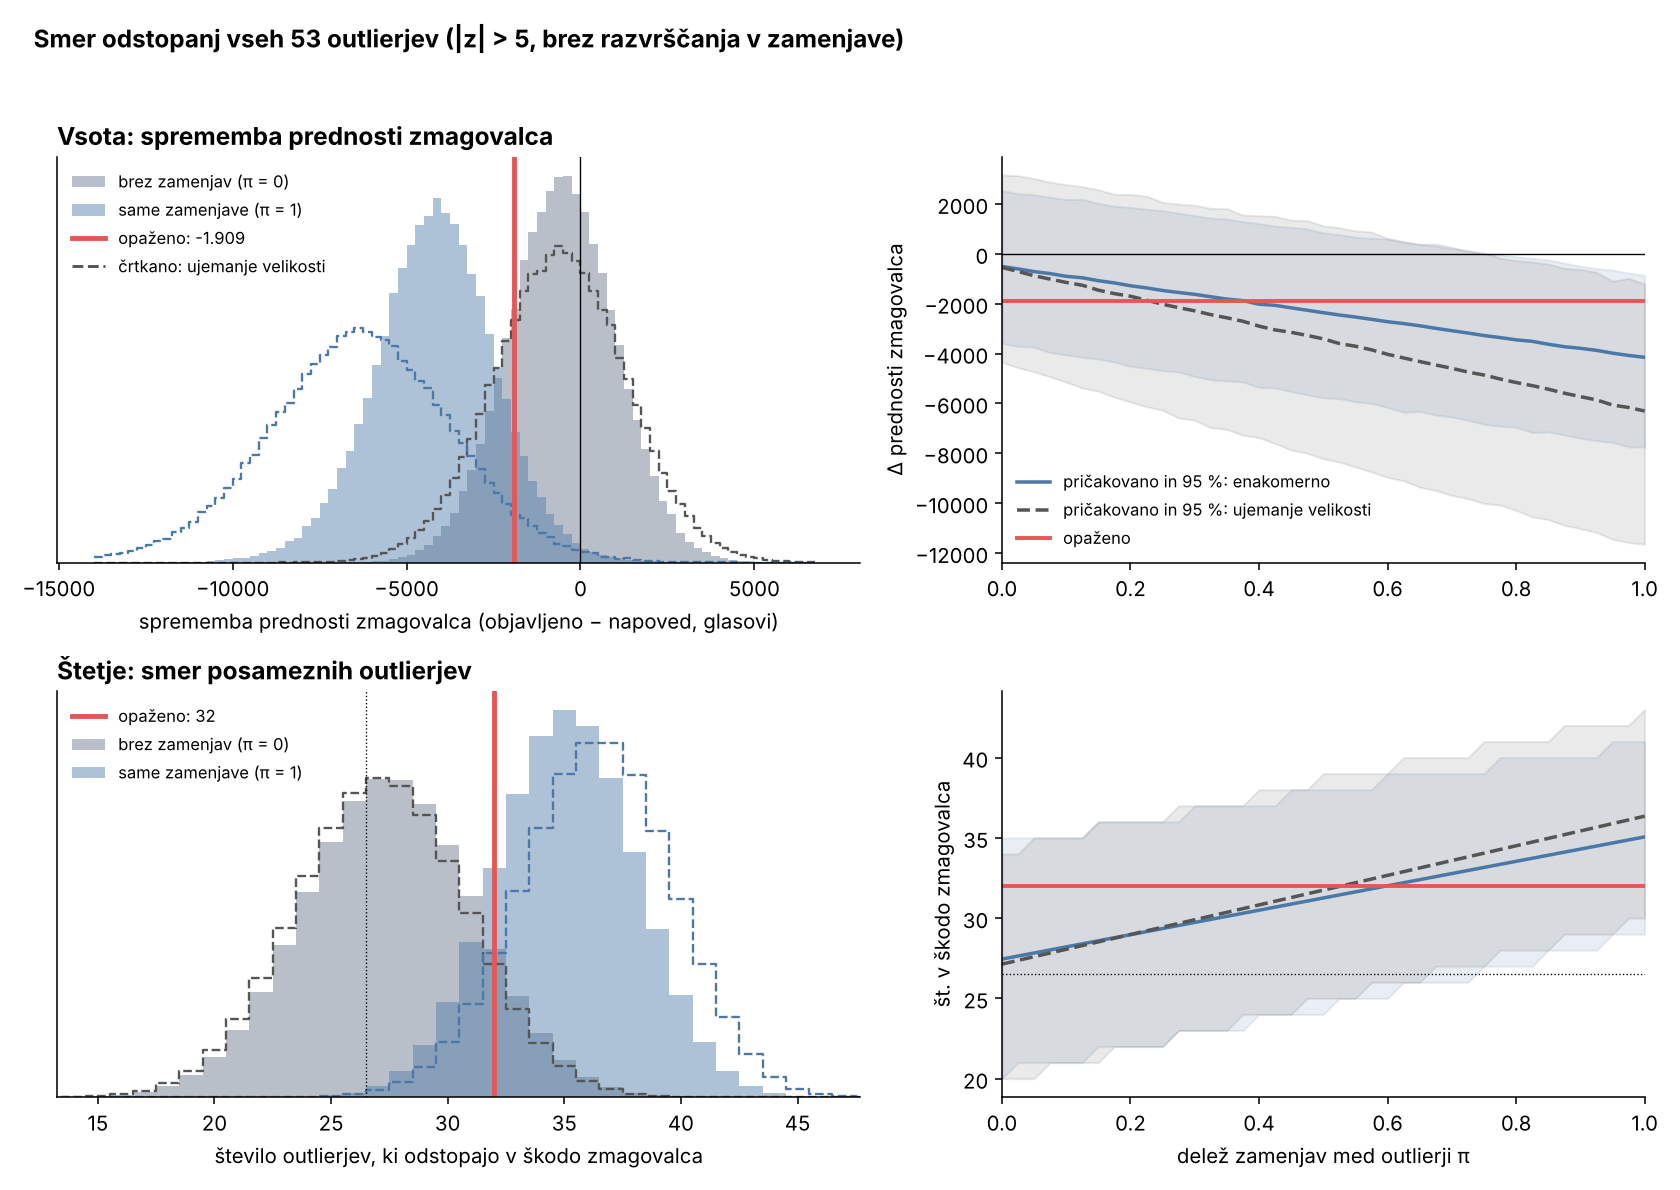
\includegraphics[width=0.95\textwidth]{15_smer_vsi_outlierji.png}
\caption{Smer odstopanj vseh 53 outlierjev, brez razvrščanja v zamenjave. Zgoraj: vsota (sprememba prednosti zmagovalca v glasovih, objavljeno minus napoved); spodaj: štetje (število outlierjev, ki odstopajo v škodo zmagovalca). Levo: porazdelitev pri hipotezi brez zamenjav ($\pi=0$, sivo) in pri hipotezi, da so vsi outlierji zamenjave ($\pi=1$, modro); stolpci: enakomerno vzorčenje volišč, črtkano: vzorčenje z enako porazdelitvijo velikosti kot pri opaženih outlierjih; rdeče opaženo. Desno: pričakovanje in 95-\% interval v odvisnosti od deleža zamenjav $\pi$. Opaženo leži med obema skrajnostma, zato smer deleža zamenjav ne omeji.}
\label{fig:smer}
\end{figure}

\textbf{Sklep.} Smer posamezne napake določa lokalna večina na volišču, skupno smer pa utežena vsota lokalnih prednosti, ki je enaka nacionalni prednosti zmagovalca; ne politična opcija. Prirejanje bi sistematično koristilo isti opciji prek vseh referendumov; tu pa napake koristijo poraženi strani, ki je pri različnih referendumih različna opcija, in izida ne spremenijo. Praktična posledica je, da tovrstne napake izid v pričakovanju prikažejo tesnejši, kot je bil.

%=====================================================
\section{Interpretacija in omejitve}

\textbf{Zakaj sum na napako in ne resnična posebnost ali prevara.} Za obstoj zamenjav govori več argumentov, ki uporabljajo različne ničelne hipoteze in različne izbore celic:
\begin{itemize}
\item \textbf{Zgoščevanje v pasu zamenjav} (razdelka~4.2 in~4.3): 27 od 53 outlierjev leži v pasu $|z^{\text{zam}}|<3$, ob naključnih odstopanjih pa jih pričakujemo 7--9 ($p\approx10^{-7}$--$10^{-8}$). Znotraj pasu se kopičijo pri 0 (17 pri $|z^{\text{zam}}|<1$ proti pričakovanim 2,5), kot to velja za binomski šum okoli pravega rezultata.
\item \textbf{Zgoščevanje ob zrcalni osi čez vse celice} (razdelek~\ref{sec:zrcalnaos}): pri razmiku nad $4\sigma$ leži ob osi 21 celic, pričakovano 4,4 iz empirične porazdelitve vseh podatkov ($p\approx10^{-8}$), brez kakršne koli razvrstitve.
\item \textbf{Oblika porazdelitve $\lambda$} (razdelek~\ref{sec:lambda}): vrh pri $\lambda=1$ med vsemi outlierji, izbranimi samo po $|z|>5$ (test razmerja verjetij, $p<10^{-10}$), robusten na mehanizem ozadja in na velikost volišča. Potrdi ga tudi test gladkosti brez modela ozadja ($p\approx3\cdot10^{-6}$).
\item \textbf{Volišča v isti stavbi} (razdelek~\ref{sec:stavba}): pri sedmih od osmih domnevnih zamenjav sestrska volišča glasujejo v skladu z napovedjo.
\item \textbf{Smer odstopanj} (razdelek~\ref{sec:smer}): skladna z ocenjenim deležem zamenjav, a brez moči ($p\approx0{,}12$--$0{,}24$).
\end{itemize}
Prvi trije argumenti niso statistično neodvisni, saj vsi temeljijo na istih outlierjih blizu zrcalne vrednosti. So pa neodvisni po metodi: pridejo do istega sklepa z različnimi predpostavkami in brez njih, zato je malo verjetno, da bi bil sklep posledica izbire ene od metod. Nobena analiza ne govori proti obstoju zamenjav kot pojava.

\textbf{Bistvo argumenta.} Vprašanje, zakaj je outlierjev več, kot predvideva normalna porazdelitev, ima lahko več nedolžnih odgovorov: resnične posebnosti posameznih volišč, porazdelitev z debelejšimi repi od predpostavljene, nenatančen model. Noben od teh odgovorov pa ne pojasni, \emph{kje} outlierji ležijo. Resnična posebnost premakne rezultat volišča za količino, ki nima zveze z oddaljenostjo napovedi od 50~\%; debelejši repi razširijo porazdelitev odstopanj, ne ustvarijo pa vrha na točno določeni vrednosti. Zrcalna vrednost $100-\hat p$ je za vsako volišče drugačna, zato bi se morala resnična posebnost na vsakem volišču posebej ``uglasiti'' nanjo do natančnosti binomskega šuma. Opaženo zgoščevanje na tem območju (17 outlierjev v jedru $\lambda\in[0{,}9;\,1{,}1]$ pri pričakovanih 2--4, ne glede na mehanizem ozadja in velikost volišč) je težko razložiti brez mehanizma, ki deluje prav na zrcalno vrednost, in najverjetnejši znani tak mehanizem je zamenjava števil ZA in PROTI. Ostale značilnosti se ujemajo z administrativno napako: smer zamenjav je skladna z naključjem (razdelek~\ref{sec:smer}), pri vseh štirih referendumih, razpršene so po okrajih, število glasovnic je skladno, vpliv je zanemarljiv in napako je trivialno odkriti iz zapisnika. Statistika sama prevare ne more izključiti, nobena značilnost podatkov pa nanjo ne kaže.

\textbf{Kje bi lahko nastala napaka.} Okrajne volilne komisije rezultate vnašajo iz zapisnikov volilnih odborov in jih še na volilni dan primerjajo z zapisniki. Če domnevne zamenjave po tem preverjanju ostanejo, bi bile lahko že v zapisniku volilnega odbora (število ZA vpisano v rubriko PROTI). Kontroli ``vnos = zapisnik'' in ``veljavne + neveljavne = oddane'' take napake ne ujameta, zato bi lahko ostala tudi v uradnih rezultatih, če je nihče ne opazi. Iz teh podatkov ni mogoče ločiti napake v zapisniku od napake pri vnosu.

\textbf{Omejitve.}
\begin{itemize}
\item Podatki so preliminarni (trenutni), ne uradni.
\item Pragi ($|z|>5$, $|z^{\text{zam}}|<3$) so hevristični; ocenjeno 2--4 lažnih zadetkov med zamenjavami.
\item Napaka je pripisana referendumu, ki se ne ujema z ostalimi tremi; pri večkratnih napakah na istem volišču je to manj zanesljivo.
\item Zamenjave pri deležih blizu 50~\% so nevidne; ocenjeno število je spodnja meja.
\item Izračun učinka na izid je pogojen na označene zamenjave; nepogojni test smeri ima nizko moč.
\item Rezultati utemeljujejo sum, ne dokazujejo napak. Najmočnejši argument za obstoj zamenjav je oblika porazdelitve $\lambda$; ostali testi so skladni, a šibki ali od nje odvisni.
\item Geografska razvrstitev (mesto/podeželje) je ročna ocena po imenih krajev.
\item Nepojasnjeni primeri so lahko drugačne napake ali resnične posebnosti (predčasna glasovanja, posebne skupnosti).
\end{itemize}

\textbf{Preverljivost.} Hipotezo je mogoče preveriti postopno. Najprej se pregledajo tri volišča, pri katerih je zamenjava po modelu najverjetnejša: PGD Bizovik (sociala), Dom kulture Braslovče~II (sociala) in OŠ Mali Slatnik (tujci). Pri vseh treh je verjetnost, da gre za zamenjavo, okoli 0,85 (konzervativna ocena mešanega modela). Pregled pomeni primerjavo objave z zapisnikom volilnega odbora in, če se ujemata, ponovno štetje glasovnic. Če je hipoteza o zamenjavah pravilna, je verjetnost, da pri nobenem od treh volišč ne najdemo napake, okoli 0,003, zato bi tak izid hipotezo ovrgel. Če zamenjav ni in so outlierji resnične posebnosti, bi zrcalno napako lahko našli le po naključju. Tudi ob velikodušni predpostavki, da ima 1~\% vseh celic zamenjavo neodvisno od označb modela, je verjetnost vsaj ene najdene napake 0,03, vsaj dveh pa 0,0003.

Že ena ali dve potrjeni zamenjavi bi zato zavrnili hipotezo ``ni zamenjav'' in upravičili pregled vseh 26 označenih volišč. Model napoveduje, da bi jih bilo potrjenih okoli 20; ujemanje tega števila bi dodatno preverilo, ali je model pravilno umerjen. Izračun predpostavlja, da so verjetnosti iz modela približno pravilne in da so napake na različnih voliščih neodvisne. Seznam volišč in pravila odločanja morajo biti objavljeni pred pregledom, da se merila ne prilagajajo izidu. Zapisnik, ki se ujema z objavo, sam še ne ovrže zamenjave, saj je ta lahko nastala že pri štetju ali vpisu v zapisnik; za ovržbo je zato potrebno ponovno štetje glasovnic.

%=====================================================
\clearpage
\addcontentsline{toc}{section}{Viri}
\begin{thebibliography}{9}
\bibitem{wand2001} J.\,N. Wand, K.\,W. Shotts, J.\,S. Sekhon, W.\,R. Mebane Jr., M.\,C. Herron, H.\,E. Brady. The Butterfly Did It: The Aberrant Vote for Buchanan in Palm Beach County, Florida. \emph{American Political Science Review} 95(4):793--810, 2001. \url{https://doi.org/10.1017/S000305540040002X}
\bibitem{mebane2004} W.\,R. Mebane Jr., J.\,S. Sekhon. Robust Estimation and Outlier Detection for Overdispersed Multinomial Models of Count Data. \emph{American Journal of Political Science} 48(2):392--411, 2004. \url{https://doi.org/10.1111/j.0092-5853.2004.00077.x}
\bibitem{ahlback2025} J. Ahlbäck, R.\,S. Jablonski. How to Distinguish Human Error from Election Fraud: Evidence from the 2019 Malawi Election. \emph{British Journal of Political Science} 55, 2025. \url{https://doi.org/10.1017/S0007123425100951}
\bibitem{okfn2014} N.\,E. Kaaber Rasmussen. Open Electoral Data Reveal Errors in Danish Electoral Results. Open Knowledge Denmark, 28.\,5.\,2014. \url{https://dk.okfn.org/index.html?p=127.html}
\bibitem{oagnz2024} Office of the Auditor-General New Zealand. \emph{General Election 2023: Independent review of counting errors}. 7.\,5.\,2024. \url{https://oag.parliament.nz/2024/election-2023/}
\end{thebibliography}

\appendix
\section{Seznam izstopajočih celic}

Seznam vseh 53 celic, ki so izstopajoče v obeh modelih ($|z|>5$), razvrščenih po tipu odstopanja. Stolpci:
\begin{itemize}\setlength{\itemsep}{0pt}
\item \textbf{Okraj, ID, Volišče}: volilni okraj, številka volišča v okraju (901 je predčasno glasovanje) in ime volišča.
\item \textbf{Ref.}: referendum, pri katerem celica izstopa.
\item \textbf{Glasov}: število veljavnih glasov na tem referendumu.
\item \textbf{ZA objav.}: objavljeni delež ZA v \%.
\item \textbf{ZA napov.}: napoved deleža ZA v \% iz ostalih treh referendumov na istem volišču (model brez FE).
\item \textbf{$z$, $z_{\text{FE}}$}: standardizirano odstopanje objavljenega deleža od napovedi v modelu brez oziroma s fiksnimi učinki okraja (enačba~\ref{eq:z}); pozitivno pomeni več ZA, kot je napovedano.
\item \textbf{$z^{\text{zam}}$}: odstopanje, če bi ZA in PROTI zamenjali (enačba~\ref{eq:zzam}, model brez FE); vrednost blizu 0 pomeni, da se zamenjani rezultat ujema z napovedjo.
\item \textbf{Kor.}: smer odstopanja; ``ZA'' pomeni, da je objavljenih glasov ZA več, kot jih napoveduje model (ali kot bi jih bilo po zamenjavi).
\item \textbf{$\Delta$ZA}: pri domnevni zamenjavi ZA$\leftrightarrow$PROTI razlika objavljeni ZA $-$ pravi ZA (če je zamenjava prava); pri ostalih ($\approx$) grob presežek glasov ZA glede na napoved.
\end{itemize}
Maribor~5/17 je med nepojasnjenimi, ker enojna zamenjava ne zadošča; razlaga s trojno zamenjavo je v razdelku~\ref{sec:veckratne}.

{\scriptsize
\setlength{\tabcolsep}{2pt}
\begin{longtable}{>{\raggedright\arraybackslash}p{2.3cm}r>{\raggedright\arraybackslash}p{3.2cm}lrrrrrrlr}
\toprule
Okraj & ID & Volišče & Ref. & Glasov & \shortstack{ZA\\objav.} & \shortstack{ZA\\napov.} & $z$ & $z_{\text{FE}}$ & $z^{\text{zam}}$ & Kor. & $\Delta$ZA \\
\endhead
\midrule
\multicolumn{12}{l}{\textbf{Domnevne zamenjave ZA$\leftrightarrow$PROTI} (26)}\\
\midrule
4005 - Ljubljana Moste-P & 27 & PGD Bizovik & Sociala & 758 & 33 & 68 & -23.7 & -26.6 & -0.5 & PROTI & -256 \\
5005 - Žalec 2 & 37 & Dom kulture Braslovče II & Sociala & 597 & 34 & 65 & -18.5 & -21.2 & +0.7 & PROTI & -191 \\
6003 - Novo Mesto 2 & 9 & OŠ Mali Slatnik & Tujci & 754 & 37 & 62 & -17.8 & -20.2 & +0.7 & PROTI & -200 \\
5003 - Celje 2 & 901 & Predčasno glasovanje & Sociala & 1375 & 61 & 40 & +18.9 & +19.7 & -0.7 & ZA & +303 \\
8010 - Ptuj 2 & 24 & DK Turnišče & Sociala & 278 & 31 & 72 & -17.7 & -19.1 & -0.9 & PROTI & -108 \\
2004 - Koper 1 & 22 & SEPŠ & Preiskava & 323 & 65 & 36 & +14.0 & +16.2 & -0.6 & ZA & +95 \\
3001 - Logatec & 30 & OŠ 8 talcev Logatec & Sociala & 943 & 40 & 60 & -14.5 & -15.2 & -0.1 & PROTI & -185 \\
3006 - Ljubljana Vič-Rud & 31 & Obrtna zbornica Vič & RTV & 568 & 62 & 40 & +11.0 & +14.7 & -0.8 & ZA & +138 \\
4007 - Ljubljana Moste-P & 18 & Park Kodeljevo-Šport Lj. (mala d & Preiskava & 277 & 65 & 37 & +13.0 & +14.4 & -0.7 & ZA & +83 \\
1001 - Jesenice & 901 & Predčasno glasovanje & Sociala & 1004 & 59 & 43 & +11.4 & +14.0 & -1.7 & ZA & +176 \\
4010 - Domžale 1 & 22 & Podružnična šola Blagovica & Preiskava & 260 & 36 & 63 & -12.1 & -13.4 & +0.2 & PROTI & -72 \\
1006 - Kranj 3 & 31 & Srednja vas & Tujci & 404 & 38 & 58 & -10.1 & -13.3 & +2.3 & PROTI & -100 \\
8007 - Lenart & 15 & OŠ Lenart & Preiskava & 152 & 34 & 70 & -12.8 & -13.2 & -1.1 & PROTI & -50 \\
2005 - Koper 2 & 5 & OŠ Elvire Vatovec Prade & RTV & 564 & 62 & 39 & +10.8 & +11.9 & -0.5 & ZA & +132 \\
6003 - Novo Mesto 2 & 901 & Predčasno glasovanje & Sociala & 810 & 58 & 41 & +11.4 & +11.4 & +0.5 & ZA & +130 \\
6005 - Brežice & 8 & (II)SIC Brežice & RTV & 252 & 62 & 37 & +8.3 & +9.6 & +0.5 & ZA & +60 \\
8004 - Murska Sobota 1 & 17 & Vaško-gasilski dom Gederovci & Sociala & 80 & 26 & 64 & -8.3 & -9.5 & +2.1 & PROTI & -38 \\
8004 - Murska Sobota 1 & 74 & Podružnična šola Krog & Tujci & 508 & 43 & 59 & -9.3 & -8.4 & -0.8 & PROTI & -76 \\
1008 - Škofja Loka 1 & 5 & Društvo upokojencev & RTV & 455 & 59 & 44 & +6.5 & +8.6 & -1.3 & ZA & +83 \\
2006 - Sežana & 1 & Avber & Tujci & 123 & 63 & 38 & +6.9 & +8.0 & -0.2 & ZA & +31 \\
8004 - Murska Sobota 1 & 107 & Vaško-gasilski dom Sotina & Sociala & 94 & 37 & 66 & -6.8 & -7.8 & -0.7 & PROTI & -24 \\
1001 - Jesenice & 32 & TVD Partizan Žirovnica & Sociala & 336 & 43 & 60 & -7.5 & -7.6 & -1.3 & PROTI & -48 \\
5002 - Celje 1 & 3 & Sedež MČ Hudinja & Sociala & 405 & 44 & 58 & -6.8 & -7.6 & -0.8 & PROTI & -51 \\
4005 - Ljubljana Moste-P & 24 & OŠ Sostro & Preiskava & 379 & 58 & 45 & +6.8 & +6.9 & -1.9 & ZA & +63 \\
5010 - Ravne Na Koroškem & 2 & Koroška kmetijska zadruga & Preiskava & 384 & 55 & 43 & +6.2 & +6.4 & +1.1 & ZA & +38 \\
6002 - Novo Mesto 1 & 41 & GD Gorenja Stara vas & Preiskava & 90 & 36 & 55 & -5.0 & -5.6 & +2.3 & PROTI & -26 \\
\midrule
\multicolumn{12}{l}{\textbf{Morda zamenjava} (1)}\\
\midrule
3005 - Ljubljana Vič-Rud & 4 & OŠ Vič & Sociala & 439 & 60 & 44 & +7.6 & +5.8 & -2.2 & ZA & $\approx$+87 \\
\midrule
\multicolumn{12}{l}{\textbf{Odstopanje pri več referendumih na istem volišču} (5)}\\
\midrule
4005 - Ljubljana Moste-P & 25 & OŠ Sostro & Preiskava & 471 & 55 & 37 & +10.4 & +10.9 & +4.7 & ZA & $\approx$+82 \\
4005 - Ljubljana Moste-P & 25 & OŠ Sostro & RTV & 471 & 37 & 52 & -6.5 & -6.6 & +4.4 & PROTI & $\approx$-71 \\
4005 - Ljubljana Moste-P & 25 & OŠ Sostro & Tujci & 471 & 73 & 55 & +9.9 & +12.8 & -15.1 & ZA & $\approx$+87 \\
1008 - Škofja Loka 1 & 6 & Zdravstveni dom Škofja Loka & RTV & 510 & 70 & 53 & +7.7 & +9.3 & -10.6 & ZA & $\approx$+87 \\
1008 - Škofja Loka 1 & 6 & Zdravstveni dom Škofja Loka & Tujci & 508 & 70 & 60 & +5.9 & +5.9 & -16.8 & ZA & $\approx$+53 \\
\midrule
\multicolumn{12}{l}{\textbf{Nepojasnjeno} (21)}\\
\midrule
4002 - Ribnica-Dobrepolj & 901 & Predčasno volišče - UE Ribnica & Preiskava & 557 & 24 & 47 & -14.4 & -16.8 & +18.4 & PROTI & $\approx$-127 \\
3005 - Ljubljana Vič-Rud & 19 & OŠ Vrhovci & Sociala & 480 & 28 & 48 & -10.4 & -11.9 & +12.0 & PROTI & $\approx$-98 \\
2005 - Koper 2 & 1 & OŠV Ankaran & Tujci & 460 & 65 & 45 & +10.4 & +11.6 & -5.5 & ZA & $\approx$+91 \\
4004 - Ivančna Gorica & 4 & KD MULJAVA & Preiskava & 451 & 87 & 70 & +10.7 & +11.3 & -34.8 & ZA & $\approx$+79 \\
7009 - Maribor 5 & 17 & OŠ Draga Kobala & Preiskava & 196 & 68 & 42 & +9.6 & +11.2 & -3.8 & ZA & $\approx$+50 \\
1006 - Kranj 3 & 21 & Naklo II & Sociala & 724 & 86 & 75 & +8.3 & +9.8 & -44.1 & ZA & $\approx$+83 \\
3007 - Ljubljana Center & 17 & OŠ Vodmat & Preiskava & 356 & 44 & 27 & +9.4 & +9.6 & +16.4 & ZA & $\approx$+60 \\
5008 - Velenje 2 & 24 & Dom krajanov Pesje & Sociala & 543 & 82 & 67 & +8.3 & +9.4 & -28.4 & ZA & $\approx$+78 \\
7002 - Slovenska Bistric & 39 & Društvo delovnih invalidov & Preiskava & 320 & 47 & 65 & -9.4 & -9.1 & -6.0 & PROTI & $\approx$-60 \\
1008 - Škofja Loka 1 & 11 & Gasilski dom Gosteče & Sociala & 258 & 93 & 74 & +8.3 & +9.3 & -29.0 & ZA & $\approx$+50 \\
4007 - Ljubljana Moste-P & 2 & OŠ Nove Jarše & RTV & 562 & 18 & 34 & -8.1 & -9.0 & +23.5 & PROTI & $\approx$-92 \\
2005 - Koper 2 & 901 & Predčasno glasovanje & Sociala & 879 & 27 & 38 & -7.6 & -8.0 & +24.7 & PROTI & $\approx$-93 \\
3008 - Ljubljana Šiška 1 & 22 & Vrtec Najdihojca & Preiskava & 364 & 28 & 18 & +6.9 & +7.6 & +36.0 & ZA & $\approx$+38 \\
8005 - Murska Sobota 2 & 23 & Večnamenska dvorana Pušča & RTV & 127 & 32 & 13 & +6.6 & +7.0 & +18.4 & ZA & $\approx$+25 \\
4005 - Ljubljana Moste-P & 901 & Predčasno glasovanje & Preiskava & 780 & 37 & 29 & +6.9 & +6.7 & +27.8 & ZA & $\approx$+65 \\
3001 - Logatec & 24 & GD Medvedje Brdo & RTV & 103 & 89 & 65 & +5.1 & +6.4 & -11.6 & ZA & $\approx$+25 \\
1007 - Tržič & 5 & Kovor & Tujci & 732 & 66 & 57 & +5.9 & +6.2 & -15.8 & ZA & $\approx$+64 \\
2007 - Ilirska Bistrica & 901 & Predčasno glasovanje & Tujci & 527 & 44 & 36 & +5.0 & +6.2 & +12.1 & ZA & $\approx$+45 \\
7011 - Maribor 7 & 901 & Predčasno glasovanje & Sociala & 583 & 31 & 40 & -5.5 & -6.0 & +16.5 & PROTI & $\approx$-56 \\
2008 - Postojna & 37 & Dom krajanov Bolk & Tujci & 243 & 69 & 55 & +5.4 & +6.0 & -9.0 & ZA & $\approx$+34 \\
8001 - Lendava & 2 & Medgeneracijski center (Bukovje) & Tujci & 156 & 58 & 74 & -5.8 & -5.5 & -11.2 & PROTI & $\approx$-26 \\
\bottomrule
\end{longtable}
}

\end{document}
